\chapter{Paths, cycles and flows in graphs} 
\label{cha:short-paths-graphs}


Suppose you want to find a shortest path from a given starting point
to a given destination. This is a common scenario in driver assistance
systems (GPS) and can be modeled as one of the most basic
combinatorial optimization problems, the \emph{shortest path problem}.
In this chapter, we introduce directed graphs, shortest paths and
flows in networks. We focus in particular on the maximum-flow problem,
which is a linear program that we solve with direct methods, versus
the simplex method, and analyze the running time of these direct
methods.

% \section{Growth of functions}
% \label{sec:growth-functions}


% In the analysis of algorithms, it is more appropriate to  investigate
% the asymptotic running time 
% of an  algorithm depending on the input and not the
% precise running time itself. We review the $O,\Omega$ and $\Theta$-notation. 

% \begin{definition}[$O,\Omega,\Theta$-notation]
  
%   Let $T,f: \setN \to \setN$ be two functions 
%   \begin{itemize}
%   \item $T(n)$ is  in $O(f(n))$, if there exist positive  constants   $n_o\in \setN$ and  $c\in\setR_{>0}$
%     with $T(n) \leq c \cdot f(n)$ for all $n\geq n_0$. 
%   \item $T(n)$ is in $\Omega(f(n))$, if there exist constants   $n_o\in \setN$ and  $c\in\setR_{>0}$
%     with $T(n) \geq c \cdot f(n)$ for all $n\geq n_0$.  
%   \item $T(n)$ is in $\Theta(f(n))$  if $T(n)$ is both  in $O(f(n))$ and 
%     in $\Omega(f(n))$. 
%   \end{itemize}
% \end{definition}



% \begin{example}
%   The function $T(n)=2n^2 + 3n +1$ is in $O(n^2)$, since for all
%   $x\geq1$ one has $2n^2 + 3n + 1 \leq 6n^2$. Here   $n_0 = 1$ and $c =
%   6$.

%   Similarly $T(n) = \Omega(n^2)$, since for each $n\geq1$ one has $2n^2 + 3n
%   +1\geq n^2$. Thus $T(n)$ is in $\Theta(n^2)$. 
% \end{example}




\section{Graphs}
\label{sec:graphs}


\begin{definition}
  \label{def:3}
  A \emph{directed  graph} is a tuple $G = (V,A)$, where $V$ is a finite set of elements, called the
    \emph{vertices} of $G$ and  $A\subseteq(V\times V)$ is the set of
  \emph{arcs} of $G$. We denote an arc by its two defining nodes $(u,v) \in
  A$. The nodes $u$ and $v$ are called  \emph{tail}  and  \emph{head}
  of the arc $(u,v)$ respectively. 
\end{definition}



\begin{figure}
  \centering 
  \tikzstyle{vertex}=[circle,fill=black!25,minimum size=15pt,inner sep=0pt]
   \tikzstyle{selected vertex} = [circle,fill=black!25,minimum size=15pt,inner sep=0pt]
   \tikzstyle{edge} = [draw,thick,->]
   \tikzstyle{weight} = [font=\small]
   \tikzstyle{selected edge} = [draw,thick, ->,blue!50]
   \tikzstyle{ignored edge} = [draw,line width=5pt,-,black!20]
   
   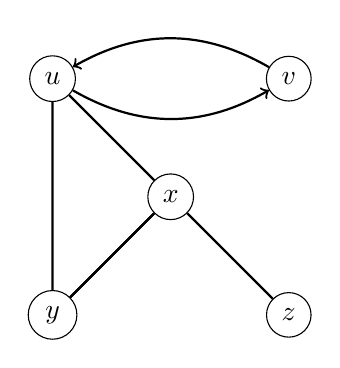
\begin{tikzpicture}[scale=1.5, auto,swap]
     \foreach \pos/\name in {{(2,1)/u}, {(4,1)/v},
       {(3,0)/x}, {(2,-1)/y}, {(4,-1)/z}}
     \node[vertex] (\name) at \pos {$\name$};
     
     \foreach \source/ \dest  in { u/y, x/u, y/x, z/x, x/y}
     \path[edge] (\source) --   (\dest);

     
     \path  (u) edge [bend right, ->, thick] (v);
     
     \path  (v) edge [bend right, ->, thick] (u);
     
   \end{tikzpicture}
   
  \caption{Example of a directed graph with $5$ nodes and $7$ arcs.}
\label{ex:graph}
\end{figure}




\begin{definition}[Walk, path, distance]
  \label{f:def:6}
  A \emph{walk} is a sequence of the form
  $$P=(v_0,a_1,v_1,\ldots,v_{m-1},a_m,v_m),$$ where  $a_i =
  (v_{i-1},v_i)\in A$ for $i=1,\ldots,m$. If the nodes $v_0,\ldots,v_m$ are all
  different, then $P$ is a \emph{path}. The \emph{length } of $P$ is
  $m$. The \emph{distance} of two nodes  $u$ and $v$ is the length of
  a shortest path from $u$ to $v$. It is denoted by $d(u,v)$. 
\end{definition}


\begin{example}
  The following is a walk and a path of the graph in
  Figure~\ref{ex:graph}. 
  \begin{displaymath}
    \begin{array}{c}
     z,(z,x),x,(x,u),u,(u,v),v,(v,u),u,(u,y),y,(y,x),x\\
     y,(y,x),x,(x,u),u,(u,v),v\\
    \end{array}
  \end{displaymath}
\end{example}


% \begin{figure}
%   \centering
%  $\psmatrix[colsep=0.2cm,mnode=circle]
% v_0&v_1 & v_3 & v_4 & v_5 & v_6 &   & v_0&v_1 & v_3 & v_4 & v_5 & v_6 \\
% \ncline{->}{1,1}{1,2}
% \ncline{->}{1,2}{1,3}
% \ncarc[arcangle=30]{->}{1,3}{1,2}
% \ncarc[arcangle=30]{->}{1,5}{1,1}
% \ncline{->}{1,3}{1,4}  
% \ncline{->}{1,4}{1,5}  
% \ncline{->}{1,5}{1,6}  
% \ncline{->}{1,8}{1,9}
% \ncline{->}{1,9}{1,10}
% \ncline{->}{1,10}{1,11}  
% \ncline{->}{1,11}{1,12}
% \ncline{->}{1,12}{1,13}
% \endpsmatrix
% $
%  \caption{Example of a walk and a path. }
% \end{figure} Das Beispiel 



\section{Representing graphs and computing the distance of two nodes}

\label{sec:repr-graphs-comp}

We represent a graph with $n$ vertices $v_1,\ldots,v_n$  as an array $A[v_1,\ldots,v_n]$, 
where the entry $A[v_i]$ is a pointer to a linked list of vertices, 
the \emph{neighbours of $v_i$}. $N(v_i) = \{ u \in V \colon (v_i,u) \in A\}$.

\begin{figure}
  \centering
 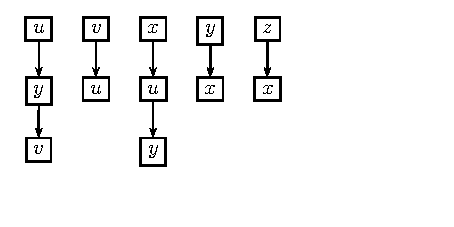
\includegraphics{figures/adjacency.pdf}
  \caption{Adjacency list representation of the graph in
    Figure~\ref{ex:graph}. } 
\end{figure}

\subsection{Breadth-first search}
\label{subsec:BFs}

We next describe a very basic algorithm that  computes the distances 
from a designated node  $s \in V$ to all other nodes. 
The \emph{distance} from $s$ to $v$ is denoted by $d(s,v)$. It is the
smallest integer $i$ such that there exists a path from $s$ to $v$ of
length $i$.  If there does not exist such a path, then  $s$ and $v$
are \emph{not connected} and we define $d(s,v) = \infty$. For $ i \in
\setN_0$,  $V_i\subseteq V$ denotes  the set of vertices that have distance $i$
from $s$.  Notice that $V_0 = \{s\}$. 

\begin{lemma}
  \label{lem:15}
  For $i=1,\ldots,n-1$, the set   $V_{i}$ is equal to the set of 
  vertices $v \in V \backslash (V_0\cup\cdots\cup V_{i-1})$ such that there exists an arc 
  $(u,v) \in A$ with $u \in V_{i-1}$.
\end{lemma}


\begin{proof}
  Suppose that $v \notin V_0\cup\cdots\cup V_{i-1}$ and there exists an arc $uv\in A$
  with $u \in V_{i-1}$. Since $u \in V_{i-1}$, there exists a path
  $s,a_1,v_1,a_2,v_2,\ldots,a_{i-1},u$ of length $i-1$ from $s$ to $u$. The
  sequence  $s,a_1,v_1,a_2,v_2,\ldots,a_i,u,uv,v$ is a path of length
  $i$ from $s$ to $v$ and thus $v \in V_{i}$. 

  If, on the other hand, $v \in V_{i}$, then there exists a path 
  \begin{displaymath}
    s,a_1,v_1,\ldots,a_{i-1},u,a_{i},v
  \end{displaymath}
  of length $i$ from $s$ to $v$. We need to show that $u \in V_{i-1}$
  holds. Clearly, since there exists a path of length $i-1$ from $s$ to
  $u$, one has $u \in V_j$ with $j\leq i-1$. If $j<i-1$, then there exists
  a path $s,a_1',v_1',\ldots,a_j',u$ of length $j$ which can be extended
  to a path of length $j+1<i$ from $s$ to $v$
  \begin{displaymath}
    s,a_1',v_1',\ldots,a_j',u,a_{i},v
  \end{displaymath}
  which contradicts $v\in V_i$.  \qed

\end{proof}


The  \emph{breadth-first search algorithm} is an implementation of
Lemma~\ref{lem:15}. 
The algorithm maintains arrays 
\begin{displaymath}
  \begin{array}{c}
    D[v_1=s,v_2,\ldots,v_n]\\
    \pi[v_1=s,v_2,\ldots,v_n]\\
  \end{array}
\end{displaymath}
and a queue $Q$ that contains only $s$ in the beginning. The array
$D$ contains at termination of the algorithm the distances from $s$ to
all other nodes and is initialized with $[0,\infty,\ldots,\infty]$.  
The array $\pi$ contains predecessor information for
shortest paths, in other words, when the algorithm terminates, $\pi[v]
= u$, where $uv$ is an arc and $D[u]+1 = D[v]$. The array $\pi$ is
initialized with $[0,\ldots,0]$.


After this initialization, the algorithm proceeds as follows. 

\begin{tabbing}
  {\bf while} \= $Q \neq \emptyset$  \\
              \> $u := head(Q)$ \\
              \> {\bf for} \= each $v \in \delta^+(u)$ \\
              \>           \> {\bf if} \= ($D[v]=\infty$) \\
              \>           \>          \> $\pi[v]:=u$ \\ 
              \>           \>          \> $D[v]:=D[u]+1$ \\
              \>           \>          \> $enqueue(Q,v)$ \\
              \> $dequeue(Q)$ 
\end{tabbing}

Here the function $head(Q)$ returns the next element in the queue and
$dequeue(Q)$ removes the first element of $Q$, while $enqueue(Q,v)$
adds $v$ to the queue $Q$ as last element.



\begin{lemma}
  \label{lem:17}
  The breadth-first search algorithm assigns \emph{distance labels} $D$
  correctly. 
\end{lemma}


\begin{proof}  
  We show the following claim by induction on $i \in \{0,\ldots,n-1\}$. 
  \begin{quote}
    For each $i \in \{1,\ldots,n-1\}$ there exists a point in time where:
    \begin{enumerate}[i)]
    \item     $Q$ contains precisely  the elements  of $V_i$
      \label{item:1}
    \item for each $v \in V_i$,  $D[v] = d(s,v)$ \label{item:2}
    \item for each $v \in V_i$  one has   $\pi[v]v$
      is an arc and $\pi[v] \in V_{i-1}$. 
    \end{enumerate}
  \end{quote}
Once this claim is shown, the lemma follows, because the labels $D[v]$
and $\pi[v]$ are only changed once, if at all, from $\infty$ or $0$ 
to an integer
or a vertex respectively. 

Since $V_0 = \{s\}$ and since  $Q = [s]$ and $D[s] = 0$ after the initialization, the
claim holds for $ i = 0$. Suppose $i>0$. By the induction hypothesis,
there is a point in time, where  $Q$ contains precisely $V_{i-1}$. By
Lemma~\ref{lem:15}, after the last element of $V_{i-1}$ is dequeued
$Q$ contains precisely the elements in $V_i$. Also, since $D[u] =
d(s,u) = i-1$ for all $u \in V_{i-1}$, we have for each $v \in V_i$ that  $D[v]
= d(s,v)=i$. Also $\pi[v]v$ is an arc, by virtue of the algorithm, and
$\pi[v] \in V_{i-1}$.  \qed 
\end{proof}

% \begin{proof}
%   Let $v \in V$. We show by induction on $d(s,v)$ that the labels are
%   correctly assigned. 

%   If $d(s,v)=0$, then $s=v$ and $D[v]=0$.  If $d(s,v)=1$, then $v$ is
%   a neighbor of $s$ and $D[v]=1$ is set correctly in the first
%   iteration of the {\bf while} loop. 
  
%   Let $d(s,v)>1$. Then there exists a $u\neq s,v$ with $d(s,u)=d(s,v)-1$
%   and $uv \in A$. By induction, the label $D[u]=d(s,u)$ is set
%   correctly by the breadth-first-search algorithm. Also, since the
%   breadth-first-search algorithm computes for $v$ a path of length
%   $D[v]$ from $s$ to $v$, the node $v$ receives a label which is
%   greater than or equal to $d(s,v)$. If we consider the sequence (over
%   time) of assigned labels, that breadth-first-search is assigning,
%   then it is easy to see that this sequence is monotonously
%   increasing, see exercise~\ref{item:16}.  The node $v$ is thus
%   explored at the latest, when $u$ is dequeued. This shows that the
%   label of $v$, $D[v]$ is assigned correctly.  \qed
% \end{proof}


\begin{definition}[Directed tree]
  \label{f:def:6}
  A \emph{directed  tree} is a directed graph $T = (V,A)$ with 
  $|A| = |V| -1$ and containing a node $r \in V$ such that there 
  exists a path from $r$ to all other nodes of $T$. 
\end{definition}



\begin{lemma}
  \label{lem:18}
  Consider the arrays $D$ and $\pi$ after the termination of the
  breadth-first-search algorithm. 
  The graph $T = (V',A')$ with $V' = \{v \in V \colon D[v]<\infty\}$ and $A' =
  \{ \pi(v) v \colon 1\leq D[v]<\infty\}$ is a tree. 
\end{lemma}


\begin{proof}
  Clearly, $|A'| = |V'| -1$. For any $i \in \{1,\ldots,n-1\}$, by
  backtracking the $\pi$-labels from any $v \in V_i$, we will eventually
  reach $s$.
\end{proof}

\begin{definition}
  \label{f:def:7}
  The tree $T$ from lemma~\ref{lem:18} is the \emph{shortest-path-tree}
   of the (unweighted) directed graph $G = (V,A)$. 
\end{definition}


% %% Adjacency matrix of graph
% %% \  a  b  c  d  e  f  g
% %% a  x  7     5
% %% b  7  x  8  9  7
% %% c     8  x     5
% %% d  5  9     x 15  6
% %% e     7  5 15  x  8  9
% %% f           6  8  x 11
% %% g              9  11 x

  \tikzstyle{vertex}=[circle,fill=black!25,minimum size=15pt,inner sep=0pt]
  \tikzstyle{selected vertex} = [vertex, fill=red!24]
  \tikzstyle{edge} = [draw,thick,->]
  \tikzstyle{weight} = [font=\small]
  \tikzstyle{selected edge} = [draw,thick, ->,blue!50]
  \tikzstyle{ignored edge} = [draw,line width=5pt,-,black!20]

 \begin{figure}
   \begin{subfigure}[t]{0.45\textwidth}
    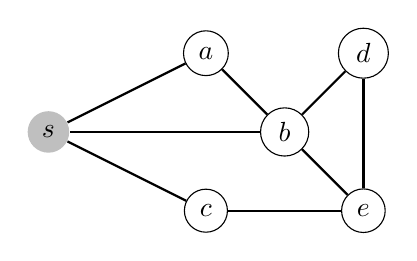
\begin{tikzpicture}[scale=1, auto,swap]
     % Draw a 7,11 network
     % First we draw the vertices
     \foreach \pos/\name in {{(2,1)/a}, {(4,1)/d},
       {(3,0)/b}, {(2,-1)/c}, {(4,-1)/e}}
     \node[vertex] (\name) at \pos {$\name$};
     
     \foreach \pos/\name in {{(0,0)/s}}
     \node[selected vertex] (\name) at \pos {$\name$};
     % Connect vertices with edges and draw weights
   
     \foreach \source/ \dest  in { s/a, s/c,
       b/s, b/d,d/e,
       b/e,e/c, a/b}
     \path[edge] (\source) --   (\dest);
     % Start animating the vertex and edge selection. 
   %   \foreach \vertex / \fr in {d/1,a/2,f/3,b/4,e/5,c/6,g/7}
 %         \path<\fr-> node[selected vertex] at (\vertex) {$\vertex$};
     % For convenience we use a background layer to highlight edges
     % This way we don't have to worry about the highlighting covering
     % weight labels. 
    %  \begin{pgfonlayer}{background}
 %         \pause
 %         \foreach \source / \dest in {d/a,d/f,a/b,b/e,e/c,e/g}
 %             \path<+->[selected edge] (\source.center) -- (\dest.center);
 %         \foreach \source / \dest / \fr in {d/b/4,d/e/5,e/f/5,b/c/6,f/g/7}
 %             \path<\fr->[ignored edge] (\source.center) -- (\dest.center);
 %     \end{pgfonlayer}
   \end{tikzpicture}
 \caption{The breadth-first search algorithm starts with the queue
   $Q=[s]$.  The distance labels for $[s,a,b,c,d,e]$ are 
   $[0,\infty,\infty,\infty,\infty,\infty]$ respectively.}
\end{subfigure}
\hfill 
\begin{subfigure}[t]{0.45\textwidth}
 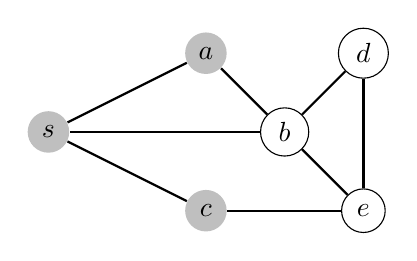
\begin{tikzpicture}[scale=1, auto,swap]
     % Draw a 7,11 network
     % First we draw the vertices
     \foreach \pos/\name in { {(4,1)/d},
       {(3,0)/b},  {(4,-1)/e}}
     \node[vertex] (\name) at \pos {$\name$};
     
     \foreach \pos/\name in {{(2,1)/a},{(2,-1)/c}, {(0,0)/s}}
     \node[selected vertex] (\name) at \pos {$\name$};
     % Connect vertices with edges and draw weights
   
     \foreach \source/ \dest  in { s/a, s/c,
       b/s, b/d,d/e,
       b/e,e/c, a/b}
     \path[edge] (\source) --   (\dest);
 \end{tikzpicture}
\caption{After the first iteration of the {\bf while} loop the queue
  is $Q = [a,c]$ and the distance labels are $[0,1,\infty,1,\infty,\infty]$ respectively. }
\end{subfigure}

\begin{subfigure}[t]{0.45\textwidth}
  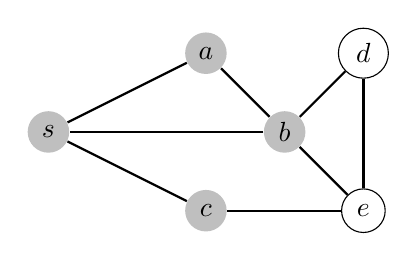
\begin{tikzpicture}[scale=1, auto,swap]
     \foreach \pos/\name in { {(4,1)/d},
        {(4,-1)/e}}
     \node[vertex] (\name) at \pos {$\name$};
     
     \foreach \pos/\name in {{(2,1)/a}, {(3,0)/b}, {(2,-1)/c}, {(0,0)/s}}
     \node[selected vertex] (\name) at \pos {$\name$};
     % Connect vertices with edges and draw weights
   
     \foreach \source/ \dest  in { s/a, s/c,
       b/s, b/d,d/e,
       b/e,e/c, a/b}
     \path[edge] (\source) --   (\dest);
  \end{tikzpicture} 
\caption{After the second iteration of the {\bf while} loop the queue
 is $Q = [c,b]$ and the distance labels are $[0,1,2,1,\infty,\infty]$ respectively. }   
\end{subfigure}
\hfill
\begin{subfigure}[t]{0.45\textwidth}
  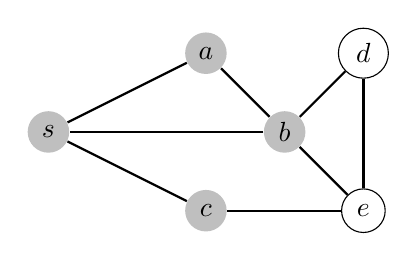
\begin{tikzpicture}[scale=1, auto,swap]
     % Draw a 7,11 network
     % First we draw the vertices
     \foreach \pos/\name in { {(4,1)/d},
        {(4,-1)/e}}
     \node[vertex] (\name) at \pos {$\name$};
     
     \foreach \pos/\name in {{(2,1)/a}, {(3,0)/b}, {(2,-1)/c}, {(0,0)/s}}
     \node[selected vertex] (\name) at \pos {$\name$};
     % Connect vertices with edges and draw weights
   
     \foreach \source/ \dest  in { s/a, s/c,
       b/s, b/d,d/e,
       b/e,e/c, a/b}
     \path[edge] (\source) --   (\dest);
  \end{tikzpicture}    
\caption{After the third iteration of the {\bf while} loop the queue
 is $Q = [b]$ and the distance labels are unchanged, since $c$ does
 not have any neighbors.  }
\end{subfigure}

\begin{subfigure}[t]{0.45\textwidth}
  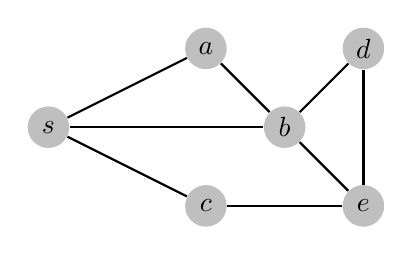
\begin{tikzpicture}[scale=1, auto,swap]
       
   \foreach \pos/\name in {{(4,1)/d},
     {(4,-1)/e}, {(2,1)/a}, {(3,0)/b}, {(2,-1)/c}, {(0,0)/s}}
   \node[selected vertex] (\name) at \pos {$\name$};
   % Connect vertices with edges and draw weights
   
   
     \foreach \source/ \dest  in { s/a, s/c,
       b/s, b/d,d/e,
       b/e,e/c, a/b}
     \path[edge] (\source) --   (\dest);
  \end{tikzpicture}    
\caption{{After the fourth iteration of the {\bf while} loop the queue
 is $Q = [d,e]$ and the distance labels are  $[0,1,2,1,3,3]$ respectively. }}
\end{subfigure}
\hfill 
\begin{subfigure}[t]{0.45\textwidth}
  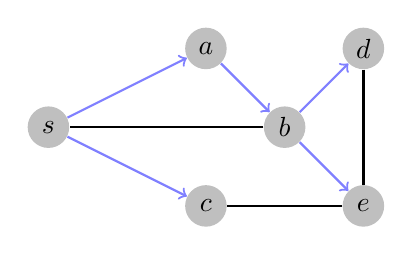
\begin{tikzpicture}[scale=1, auto,swap]
    
     \foreach \pos/\name in {{(4,1)/d},
        {(4,-1)/e}, {(2,1)/a}, {(3,0)/b}, {(2,-1)/c}, {(0,0)/s}}
     \node[selected vertex] (\name) at \pos {$\name$};
     % Connect vertices with edges and draw weights
   
     \foreach \source/ \dest  in {b/s, d/e, e/c}
     \path[edge] (\source) --   (\dest);

     
     \foreach \source/ \dest  in { s/a, s/c, b/d,  b/e, a/b}
     \path[selected edge] (\source) --   (\dest);

  \end{tikzpicture}    
\caption{After the fifth and sixth iteration of the {\bf while} loop 
 the queue is empty $Q = []$ and the distance labels remain unchanged. 
 The blue edges denote the shortest path tree.}
\end{subfigure}
  


\caption{An example-run of breadth-first search}\label{g:fig:4}
\end{figure}





\begin{theorem}
  \label{f:thr:26}
  The breath-first-search algorithm runs in time $O( |V| + |A|)$. 
\end{theorem}

\begin{proof}
  Each vertex is queued and dequeued at most once. These queuing
  operations take constant time each. Thus queuing and dequeuing costs
  $O( |V| )$ in total. 

  When a vertex $u$ is dequeued, its neighbors are
  inspected and the operations in the {\bf if} statement cost constant
  time each. Thus one has an additional cost of $O( |A | )$, since
  these constant-time  operations are carried out for each arc $a \in
  A$. 
  \qed
\end{proof}

\section{Shortest Paths}
\label{sec:shortest-paths}

\begin{definition}[Cycle]
  A walk in which starting node and end-node agree is called a
  \emph{cycle}. 
\end{definition}

Suppose we are given a directed graph $D=(V,A)$ and a length function
$c:~A\longrightarrow\setR$. The \emph{length} of a walk $W$ is defined as 
\begin{displaymath}
  c(W) = \sum_{\substack{a \in A\\ a\in W}}  c(a). 
\end{displaymath}
%
We now study how to determine a shortest path in a weighted directed
graph
$G$ efficiently, in case of the absence of cycles of negative length (such cycles are called \emph{negative cycles}). 

\begin{theorem}
  \label{f:thr:1}
  Suppose that each cycle in $D$ has non-negative length and suppose
  there exists an $s-t$-walk in $D$. Then there exists a path
  connecting $s$ with $t$ which has minimum length among all walks
  connecting $s$ and $t$. 
\end{theorem}

\begin{proof}
  If there exists an $s-t$-walk, then there exists an $s-t$-path. Since
  the number of arcs in a path is at most $|V| - 1 $, there must exist a
  shortest \emph{path}  $P$  connecting $s$ and $t$. We claim that
  $c(P)\leq c(W)$ for all $s-t$-walks $W$. Suppose that there exists
  an $s-t$-walk $W$ with $c(W)<c(P)$. Then let $W$ be such a walk with
  a minimum number of arcs. Clearly $W$ contains a cycle $C$.  Since the
  cycle has non-negative length, then it can be removed from $W$ to
  obtain a walk whose length is at most $c(W)$ and whose number of
  arcs is strictly less than $|W|$. This is a contradiction to the 
  minimality of the number of arcs in $W$.
  \qed
\end{proof}

We use the notation $|W|,|C|,|P|$ to denote the number of arcs in a
walk $W$, a cycle $C$ or a path $P$. 


As a conclusion we can note here: 
\begin{quote}
  If there do not exist negative cycles in $D$, and $s$ and $t$ are
  connected, then there exists a shortest walk traversing at most 
  $|V|  - 1$ arcs.
\end{quote}


\subsection*{The Bellman-Ford algorithm}

Let $n=|V|$. We calculate functions $f_0,f_1,\ldots,f_n:V\longrightarrow\setR\cup\{\infty\}$
successively by the following rule. 

\begin{enumerate}[i)]
\item $f_0(s) = 0$, $f_0(v) = \infty$ for all $v \neq s$ 
\item For $k<n$ if $f_k$ has been found, compute 
  \begin{displaymath}
    \displaystyle f_{k+1}(v) = \min\{f_k(v), \min_{(u,v)\in A}\{f_k(u)+c(u,v)\} \}  
  \end{displaymath}
  for all $v \in V$. 
\end{enumerate}





% %% Adjacency matrix of graph
% %% \  a  b  c  d  e  f  g
% %% a  x  7     5
% %% b  7  x  8  9  7
% %% c     8  x     5
% %% d  5  9     x 15  6
% %% e     7  5 15  x  8  9
% %% f           6  8  x 11
% %% g              9  11 x

  \tikzstyle{vertex}=[circle,fill=black!25,minimum size=15pt,inner sep=0pt]
  \tikzstyle{selected vertex} = [vertex, fill=red!24]
  \tikzstyle{edge} = [draw,thick,->]
  \tikzstyle{weight} = [font=\small]
  \tikzstyle{selected edge} = [draw,thick, ->,blue!50]
  \tikzstyle{ignored edge} = [draw,line width=5pt,-,black!20]

 \begin{figure}
 
      \begin{subfigure}[t]{0.45\textwidth}
     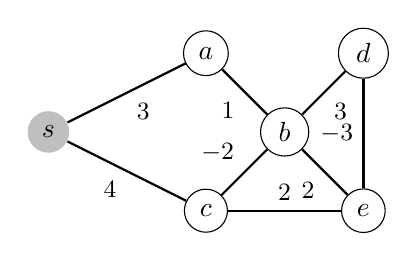
\begin{tikzpicture}[scale=1, auto,swap]
     % Draw a 7,11 network
     % First we draw the vertices
     \foreach \pos/\name in {{(2,1)/a}, {(4,1)/d},
       {(3,0)/b}, {(2,-1)/c}, {(4,-1)/e}}
     \node[vertex] (\name) at \pos {$\name$};
     
     \foreach \pos/\name in {{(0,0)/s}}
     \node[selected vertex] (\name) at \pos {$\name$};
     % Connect vertices with edges and draw weights
   
     \foreach \source/ \dest/ \weight   in { s/a/3, s/c/4,
       b/c/-2, b/d/3 ,d/e/-3,
       b/e/2,e/c/2, a/b/1}
     \path[edge] (\source) -- node[weight] {$\weight$}   (\dest);
     % Start animating the vertex and edge selection. 
   %   \foreach \vertex / \fr in {d/1,a/2,f/3,b/4,e/5,c/6,g/7}
 %         \path<\fr-> node[selected vertex] at (\vertex) {$\vertex$};
     % For convenience we use a background layer to highlight edges
     % This way we don't have to worry about the highlighting covering
     % weight labels. 
    %  \begin{pgfonlayer}{background}
 %         \pause
 %         \foreach \source / \dest in {d/a,d/f,a/b,b/e,e/c,e/g}
 %             \path<+->[selected edge] (\source.center) -- (\dest.center);
 %         \foreach \source / \dest / \fr in {d/b/4,d/e/5,e/f/5,b/c/6,f/g/7}
 %             \path<\fr->[ignored edge] (\source.center) -- (\dest.center);
 %     \end{pgfonlayer}
   \end{tikzpicture}
     
     \caption{
   The algorithm is initialized with distance labels for
   $s,a,b,c,d,e$ being $[0,\infty,\infty,\infty,\infty,\infty]$ respectively 
}
   \end{subfigure}\hfill 
      \begin{subfigure}[t]{0.45\textwidth}
      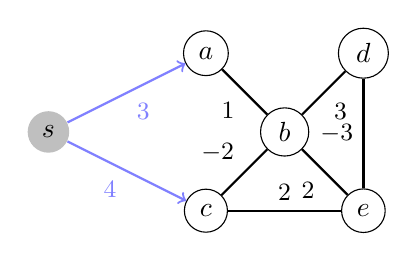
\begin{tikzpicture}[scale=1, auto,swap]
     % Draw a 7,11 network
     % First we draw the vertices
     \foreach \pos/\name in {{(2,1)/a}, {(4,1)/d},
       {(3,0)/b}, {(2,-1)/c}, {(4,-1)/e}}
     \node[vertex] (\name) at \pos {$\name$};
     
     \foreach \pos/\name in {{(0,0)/s}}
     \node[selected vertex] (\name) at \pos {$\name$};
     % Connect vertices with edges and draw weights
   
     \foreach \source/ \dest/ \weight   in {b/c/-2, b/d/3 ,d/e/-3,b/e/2,e/c/2, a/b/1}
     \path[edge] (\source) -- node[weight] {$\weight$}   (\dest);
     
     
     \foreach \source/ \dest/ \weight   in { s/a/3, s/c/4      }
     \path[selected edge] (\source) -- node[weight] {$\weight$}   (\dest);

     % Start animating the vertex and edge selection. 
   %   \foreach \vertex / \fr in {d/1,a/2,f/3,b/4,e/5,c/6,g/7}
 %         \path<\fr-> node[selected vertex] at (\vertex) {$\vertex$};
     % For convenience we use a background layer to highlight edges
     % This way we don't have to worry about the highlighting covering
     % weight labels. 
    %  \begin{pgfonlayer}{background}
 %         \pause
 %         \foreach \source / \dest in {d/a,d/f,a/b,b/e,e/c,e/g}
 %             \path<+->[selected edge] (\source.center) -- (\dest.center);
 %         \foreach \source / \dest / \fr in {d/b/4,d/e/5,e/f/5,b/c/6,f/g/7}
 %             \path<\fr->[ignored edge] (\source.center) -- (\dest.center);
 %     \end{pgfonlayer}
   \end{tikzpicture}
     
     \caption{
   After the first iteration the labels are $[0,3,\infty,4,\infty,\infty]$
}
   \end{subfigure}




      \begin{subfigure}[t]{0.45\textwidth}
      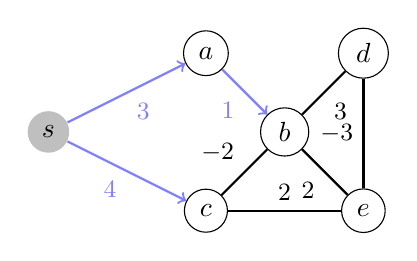
\begin{tikzpicture}[scale=1, auto,swap]
     % Draw a 7,11 network
     % First we draw the vertices
     \foreach \pos/\name in {{(2,1)/a}, {(4,1)/d},
       {(3,0)/b}, {(2,-1)/c}, {(4,-1)/e}}
     \node[vertex] (\name) at \pos {$\name$};
     
     \foreach \pos/\name in {{(0,0)/s}}
     \node[selected vertex] (\name) at \pos {$\name$};
     % Connect vertices with edges and draw weights
   
     \foreach \source/ \dest/ \weight   in {b/c/-2, b/d/3 ,d/e/-3,b/e/2,e/c/2}
     \path[edge] (\source) -- node[weight] {$\weight$}   (\dest);
     
     
     \foreach \source/ \dest/ \weight   in { s/a/3, s/c/4, a/b/1      }
     \path[selected edge] (\source) -- node[weight] {$\weight$}   (\dest);

     % Start animating the vertex and edge selection. 
   %   \foreach \vertex / \fr in {d/1,a/2,f/3,b/4,e/5,c/6,g/7}
 %         \path<\fr-> node[selected vertex] at (\vertex) {$\vertex$};
     % For convenience we use a background layer to highlight edges
     % This way we don't have to worry about the highlighting covering
     % weight labels. 
    %  \begin{pgfonlayer}{background}
 %         \pause
 %         \foreach \source / \dest in {d/a,d/f,a/b,b/e,e/c,e/g}
 %             \path<+->[selected edge] (\source.center) -- (\dest.center);
 %         \foreach \source / \dest / \fr in {d/b/4,d/e/5,e/f/5,b/c/6,f/g/7}
 %             \path<\fr->[ignored edge] (\source.center) -- (\dest.center);
 %     \end{pgfonlayer}
   \end{tikzpicture}

     
     \caption{
   After the second iteration the labels are $[0,3,4,4,\infty,\infty]$
}
   \end{subfigure}\hfill 
      \begin{subfigure}[t]{0.45\textwidth}
      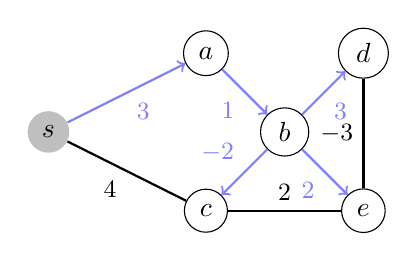
\begin{tikzpicture}[scale=1, auto,swap]
     % Draw a 7,11 network
     % First we draw the vertices
     \foreach \pos/\name in {{(2,1)/a}, {(4,1)/d},
       {(3,0)/b}, {(2,-1)/c}, {(4,-1)/e}}
     \node[vertex] (\name) at \pos {$\name$};
     
     \foreach \pos/\name in {{(0,0)/s}}
     \node[selected vertex] (\name) at \pos {$\name$};
     % Connect vertices with edges and draw weights
   
     \foreach \source/ \dest/ \weight   in {d/e/-3,e/c/2, s/c/4}
     \path[edge] (\source) -- node[weight] {$\weight$}   (\dest);
     
     
     \foreach \source/ \dest/ \weight   in {b/e/2,b/c/-2, b/d/3 , s/a/3, a/b/1      }
     \path[selected edge] (\source) -- node[weight] {$\weight$}   (\dest);

     % Start animating the vertex and edge selection. 
   %   \foreach \vertex / \fr in {d/1,a/2,f/3,b/4,e/5,c/6,g/7}
 %         \path<\fr-> node[selected vertex] at (\vertex) {$\vertex$};
     % For convenience we use a background layer to highlight edges
     % This way we don't have to worry about the highlighting covering
     % weight labels. 
    %  \begin{pgfonlayer}{background}
 %         \pause
 %         \foreach \source / \dest in {d/a,d/f,a/b,b/e,e/c,e/g}
 %             \path<+->[selected edge] (\source.center) -- (\dest.center);
 %         \foreach \source / \dest / \fr in {d/b/4,d/e/5,e/f/5,b/c/6,f/g/7}
 %             \path<\fr->[ignored edge] (\source.center) -- (\dest.center);
 %     \end{pgfonlayer}
   \end{tikzpicture}
     
     \caption{
   After the third iteration the labels are $[0,3,4,2,7,6]$
}
   \end{subfigure}





      \begin{subfigure}[t]{0.45\textwidth}
      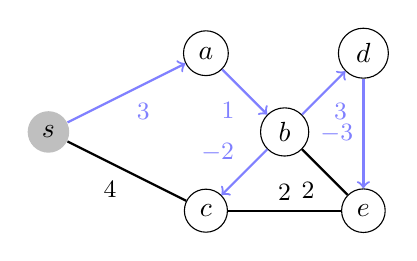
\begin{tikzpicture}[scale=1, auto,swap]
     % Draw a 7,11 network
     % First we draw the vertices
     \foreach \pos/\name in {{(2,1)/a}, {(4,1)/d},
       {(3,0)/b}, {(2,-1)/c}, {(4,-1)/e}}
     \node[vertex] (\name) at \pos {$\name$};
     
     \foreach \pos/\name in {{(0,0)/s}}
     \node[selected vertex] (\name) at \pos {$\name$};
     % Connect vertices with edges and draw weights
   
     \foreach \source/ \dest/ \weight   in { b/e/2, e/c/2, s/c/4}
     \path[edge] (\source) -- node[weight] {$\weight$}   (\dest);
     
     
     \foreach \source/ \dest/ \weight   in {d/e/-3,b/c/-2, b/d/3 , s/a/3, a/b/1      }
     \path[selected edge] (\source) -- node[weight] {$\weight$}   (\dest);

     % Start animating the vertex and edge selection. 
   %   \foreach \vertex / \fr in {d/1,a/2,f/3,b/4,e/5,c/6,g/7}
 %         \path<\fr-> node[selected vertex] at (\vertex) {$\vertex$};
     % For convenience we use a background layer to highlight edges
     % This way we don't have to worry about the highlighting covering
     % weight labels. 
    %  \begin{pgfonlayer}{background}
 %         \pause
 %         \foreach \source / \dest in {d/a,d/f,a/b,b/e,e/c,e/g}
 %             \path<+->[selected edge] (\source.center) -- (\dest.center);
 %         \foreach \source / \dest / \fr in {d/b/4,d/e/5,e/f/5,b/c/6,f/g/7}
 %             \path<\fr->[ignored edge] (\source.center) -- (\dest.center);
 %     \end{pgfonlayer}
   \end{tikzpicture}

     
     \caption{
   After the fourth iteration the labels are $[0,3,4,2,7,4]$
}
   \end{subfigure}\hfill 
      \begin{subfigure}[t]{0.45\textwidth}
      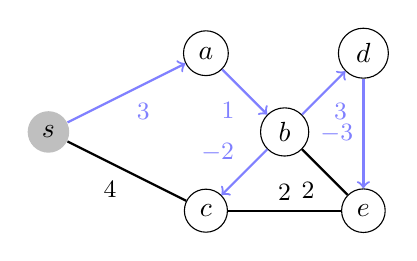
\begin{tikzpicture}[scale=1, auto,swap]
     % Draw a 7,11 network
     % First we draw the vertices
     \foreach \pos/\name in {{(2,1)/a}, {(4,1)/d},
       {(3,0)/b}, {(2,-1)/c}, {(4,-1)/e}}
     \node[vertex] (\name) at \pos {$\name$};
     
     \foreach \pos/\name in {{(0,0)/s}}
     \node[selected vertex] (\name) at \pos {$\name$};
     % Connect vertices with edges and draw weights
   
     \foreach \source/ \dest/ \weight   in { b/e/2, e/c/2, s/c/4}
     \path[edge] (\source) -- node[weight] {$\weight$}   (\dest);
     
     
     \foreach \source/ \dest/ \weight   in {d/e/-3,b/c/-2, b/d/3 , s/a/3, a/b/1      }
     \path[selected edge] (\source) -- node[weight] {$\weight$}   (\dest);

     % Start animating the vertex and edge selection. 
   %   \foreach \vertex / \fr in {d/1,a/2,f/3,b/4,e/5,c/6,g/7}
 %         \path<\fr-> node[selected vertex] at (\vertex) {$\vertex$};
     % For convenience we use a background layer to highlight edges
     % This way we don't have to worry about the highlighting covering
     % weight labels. 
    %  \begin{pgfonlayer}{background}
 %         \pause
 %         \foreach \source / \dest in {d/a,d/f,a/b,b/e,e/c,e/g}
 %             \path<+->[selected edge] (\source.center) -- (\dest.center);
 %         \foreach \source / \dest / \fr in {d/b/4,d/e/5,e/f/5,b/c/6,f/g/7}
 %             \path<\fr->[ignored edge] (\source.center) -- (\dest.center);
 %     \end{pgfonlayer}
   \end{tikzpicture}

     
     \caption{
   After the fifth  iteration the labels are unchanged. The shortest
   path distances have been computed. 
}
   \end{subfigure}
   
 \caption{An example-run of the Bellman-Ford algorithm. The blue
     edges represent the tree whose paths have the corresponding lengths.} \label{f:fig:5}

 \end{figure}




The following theorem shows us that the Bellman-Ford algorithm is a 
method to compute minimum length walks.


\begin{theorem}
  \label{f:thr:1}
  For each $k=0,\ldots,n$ and for each $v \in V$ 
  \begin{displaymath}
    f_k(v)  = \min\{ c(P) \colon  P \text{ is an } s-v\text{-walk traversing
    at most } k \text{ arcs}\}.
  \end{displaymath}
\end{theorem}

\begin{theorem}
   \label{bobo:f:thr:1}
   Given a directed graph $D=(V,A)$, $s \in V$ and a length 
   function $c:A \to \setR$, one has $f_n = f_{n-1}$ if and only 
   if $D$ does not have a cycle 
   of negative length that is reachable from $s$.
\end{theorem}

\begin{proof}
   $(\Leftarrow)$ Suppose there exists $t \in V$ such that 
   $f_n(t) < f_{n-1}(t) < \infty$. This implies that the shortest 
   $s-t$-walk traversing at most $n$ arcs (call it $W$) traverses 
   exactly $n$ arcs and thus contains a cycle (call it $C$). Consider 
   the $s-t$-walk $W'$ obtained by eliminating $C$ from $W$. 
   $W'$ traverses at most $n-1$ arcs and thus we have $c(W') > c(W)$.
   Since $c(W) = c(W') + c(C)$, we have that $c(C) < 0$.
   
   $(\Rightarrow)$ Let $C = v_0,v_1,\cdots,v_k,v_0$ be a cycle 
   reachable from $s$. Notice that 
   $f_{n-1}(v_i)<\infty$ $\forall 0 \leq i \leq k$. 
   We can show that $C$ is a non-negative cycle by these simple 
   calculations (notice that the node indices $i$ and $i+1$ are 
   considered modulo $k$ in the following sums).
   \begin{displaymath}
      0 = \sum_{i = 0}^k f_n(v_{i+1}) - f_n(v_i) \leq
      \sum_{i = 0}^k c(v_i,v_{i+1}) = c(C)
   \end{displaymath}
\end{proof}

Theorem~\ref{bobo:f:thr:1} can be generalized for every $n \geq |V|$.
This allows us to obtain the following corollary.

\begin{corollary}
  \label{co:7}
  If $D = (V,A) $ does not contain negative cycles w.r.t. $c$, then
  $f_n(v)$ is equal to the length of a shortest $s-v$-path. The
  numbers $f_n(v)$ can be computed in time $O( |V| \cdot |A| )$. 
\end{corollary}

Notice that by using theorem~\ref{bobo:f:thr:1} 
we can see if a directed graph $D(V,A)$ has negative cycles in the 
following way. We obtain a new graph $D'=(V',A')$ add a node $s$ to 
$D$ and we connect $s$ to all other vertices with an outgoing arc 
of weight $0$. Then, we apply Bellman-Ford algorithm to $D'$ with 
starting node $s$. Notice that $D$ contains a negative cycle, if 
and only if $D'$ contains a negative cycle (since every cycle in $D$ 
is reachable from $s$ in $D'$). Thus $D$ contains a 
negative cycle if and only if there exists $t \in V$ such that 
$f_n(t) < f_{n-1}(t)$ in $D'$.
This gives us the following corollary.

\begin{corollary}
  \label{co:9}
  In time $O(|V| \cdot |A| )$  one can test whether $D = (V,A)$ has a
  negative cycle w.r.t. $c$ and eventually return one. 
\end{corollary}

\begin{proof}
   By our previous words we know that we simply have to apply 
   Bellman-Ford algorithm to the graph $D'$. The corollary follows 
   by the fact that $|V'| = |V|+1$ and $|A'| = |A| + |V|$ and by 
   using corollary~\ref{co:7}.
\end{proof}

\section{Maximum $s-t$-flows}
\label{sec:maximum-s-t}

We now turn our attention to a linear programming problem which we
will solve by direct methods, motivated by the nature of the 
problem. We often use the following notation. If $f:A\longrightarrow B$ denotes a
function and if $U\subseteq A$, then $f(U)$ is defined as $f(U)= \sum_{a\in U}
f(a)$.  




\begin{definition}[Network, $s-t$-flow]
  A network with capacities  consists of a directed simple graph
  $D=(V,A)$ and a   \emph{capacity function} $u:A\to\setR_{\geq0}$. 
  We also require that if there is an arc $uv \in A$, then there is 
  no reverse arc $vu$, and we disallow self-loops. 
  A function $f:A\to\setR_{\geq0}$ is   called an \emph{$s-t$-flow}, if 
  \begin{equation}
    \sum_{e \in \delta^{out}(v)} f(e) = \sum_{e \in \delta^{in}(v)} f(e), \, \mbox{ for all } v \in V - \{s,t\},
  \end{equation}
  where $s,t\in V$. These two vertices are called \emph{source} and 
  \emph{sink} respectively. 
  The flow is \emph{feasible}, if $f(e) \leq u(e)$ for all
  $e \in A$. 
  The \emph{value} of $f$ is defined as 
  $value(f) =  \sum_{e \in \delta^{out}(s)} f(e) - \sum_{e \in \delta^{in}(s)} f(e)$.
  The \emph{maximum $s-t$-flow problem} is the problem of determining
  a maximum feasible $s-t$-flow. 
\end{definition}


Here, for $U \subseteq V$, $\delta^{in}(U)$ denotes the arcs which are entering $U$
and $\delta^{out}(U)$ denotes the arcs which are leaving $U$.   Arc sets
of the form $\delta^{out}(U)$   are called a \emph{cut} of $D$. The
\emph{capacity of a cut } $u(\delta^{out}(U))$ is the sum of the capacities of
its arcs. 


Thus the maximum  flow problem is a linear program of the form 

\begin{eqnarray}
  \max \sum_{e \in \delta^{out}(s)} x(e) & - &   \sum_{e \in \delta^{in}(s)} x(e) \\
   \sum_{e \in \delta^{out}(v)} x(e) & = &  \sum_{e \in \delta^{in}(v)} x(e), \, \mbox{ for all
   } v \in V-\{s,t\} \\
   x(e) & \leq & u (e) , \, \mbox{ for all
   } e \in A \\
   x(e) & \geq & 0 , \, \mbox{ for all
   } e \in A
\end{eqnarray}


\begin{definition}[excess function]
  For any $f:A \to \setR$, the excess function is the function 
  $excess_f:  2^V \to \setR$  defined by $excess_f(U) = \sum_{e \in \delta^{in}(U)}
  f(e) - \sum_{e \in \delta^{out}(U)} f(e)$. 
\end{definition}


\begin{theorem}
\label{f:thr:6}
Let $D = (V,A)$ be a digraph, let $f:A\to\setR$ and let $U\subseteq V$, then
\begin{equation}
  \label{f:eq:28}
  excess_f(U) = \sum_{v \in U} excess_f(v).
\end{equation}  
\end{theorem}


\begin{proof}
  An arc which has both endpoints in $U$ is counted twice with
  different parities on the right, and thus cancels out. An arc which
  has its tail in $U$ is subtracted once on the right and once on the
  left.  An arc which has its head in $U$ is added once on the right
  and once on the left. \qed
\end{proof}

A cut $\delta^{out}(U)$ with $s \in U$  and $t \notin U$ is called an $s-t$-cut.  

\begin{theorem}[Weak duality]
  \label{f:thr:7}
  Let $f$ be a feasible $s-t$-flow and let $\delta^{out}(U)$ be an
  $s-t$-cut, then $value(f) \leq u(\delta^{out}(U))$. 
\end{theorem}

\begin{proof}
  $value(f) = -excess_f(s) = -excess_f(U) = f(\delta^{out}(U)) -
  f(\delta^{in}(U)) \leq f(\delta^{out}(U)) \leq u(\delta^{out}(U))$. \qed
\end{proof}

For an arc $a = (u,v) \in A$ the arc $a^{-1}$ denotes the arc $(v,u)$. 

\begin{definition}[Residual graph]
  Let $f:A \to \setR$,  and $u: A \to \setR$ where $0 \leq f \leq u$. Consider
  the sets of arcs
  \begin{equation}
    \label{f:eq:30}
    A_f = \{ a \mid a \in A, \, f(a) < u(a)\} \cup \{ a^{-1} \mid a \in A, \, f(a) >    0\}. 
  \end{equation}
  The digraph $D(f) = (V,A_f)$ is called the \emph{residual graph} of
  $f$ (for capacities $u$).   
\end{definition}



\begin{corollary}
  \label{co:6}
  Let $f$ be a feasible $s-t$-flow and suppose that $D(f)$ has no path
  from $s$ to $t$, then $f$ has maximum value.
\end{corollary}


\begin{proof}
  Let $U$ be the set of nodes which are reachable in $D(f)$ from
  $s$. Clearly $\delta^{out}(U)$ is an $s-t$-cut. Now $value(f) = f(\delta^{out}(U)) -
  f(\delta^{in}(U)$.  Each arc leaving $U$ is not an arc of $D(f)$ and thus
  $f(\delta^{out}(U)) = u (\delta^{out}(U))$. Each arc entering $U$ does not
  carry any flow   and thus $f(\delta^{in}(U)) = 0$. It follows that  
  $value(f) = u (\delta^{out}(U))$ and $f$ is optimal by
  Theorem~\ref{f:thr:7}.   \qed
\end{proof}

\begin{definition}[undirected walk]
\label{f:def:7}
  An \emph{undirected walk} is a  sequence of the form
  $P=(v_0,a_1,v_1,\ldots,v_{m-1},a_m,v_m)$, where  $a_i \in A$ for
  $i=1,\ldots,m$ and $a_i = (v_{i-1},v_i)$ or $a_i = (v_{i},v_{i-1})$. If
  the nodes $v_0,\ldots,v_m$ are all 
  different, then $P$ is an \emph{undirected path}. 
% The \emph{length } of $P$ is
%   $m$. The \emph{distance} of two nodes  $u$ and $v$ is the length of
%   a shortest path from $u$ to $v$. 
\end{definition}


Any directed path $P$ in $D(f)$ yields an undirected path  in
$D$. Define for such a path $P$ the vector $\chi^P \in \{0,\pm1\}^A$ as
\begin{equation}
  \label{f:eq:29}
  \chi^P(a) = 
  \begin{cases}
    1 & \mbox{ if $P$ traverses $a$},\\
    -1&  \mbox{ if $P$ traverses $a^{-1}$},\\
    0 & \mbox{ if $P$ traverses neither $a$ or $a^{-1}$}. 
  \end{cases}
\end{equation}


\begin{theorem}[max-flow min-cut theorem, strong duality]
  \label{f:thr:8}
  The maximum value of a feasible $s-t$-flow is equal to the minimum
  capacity of an $s-t$ cut.
\end{theorem}

\begin{proof}
  Let $f$ be a maximum $s-t$-flow. Consider the residual graph
  $D(f)$. If this residual graph contains an 
  $s-t$-path $P$, then we can route flow along this path. More
  precisely, there exists an $\epsilon>0$ such that $f + \epsilon \, \chi^P$ is feasible.
  We have $value(f + \epsilon \, \chi^P) = value(f) + \epsilon $. This contradicts the
  maximality of $f$ thus there exists no $s-t$-path in $D(f)$. 
  
  Let $U$ be the nodes reachable from $s$ in $D(f)$. Then 
  $value(f)=u(\delta^{out}(U))$ and $\delta^{out}(U)$ is an
  $s-t$-cut of minimum capacity by the weak duality theorem.
\end{proof}
 


This suggests the algorithm of Ford and Fulkerson to find a maximum
flow. Start with $f = 0$. Next iteratively apply the following
\emph{flow augmentation algorithm}. 


Let $P$ be a directed $s-t$-path in $D(f)$. Set $f \gets f + \epsilon\chi^P$, where
$\epsilon$ is as large as possible to maintain $0\leq f\leq u$. 

\begin{exercise}
   Define a \emph{residual capacity} for $D(f)$. Then determine 
   the maximum $\epsilon$ such that $0\leq f\leq u$.
\end{exercise}

\begin{theorem}
  \label{f:thr:9}
  If all capacities are rational, this algorithm terminates. 
\end{theorem}

\begin{proof}
   By multiplying all the capacities by $10^x$ with $x$ 
   sufficiently large, we can suppose the capacities to be 
   integral. Since the value of the flow is augmented at 
   every step at least by $1$ and the capacities are finite, our 
   algorithm finds a maximum flow in finitely many iterations.
\end{proof}


\begin{center}
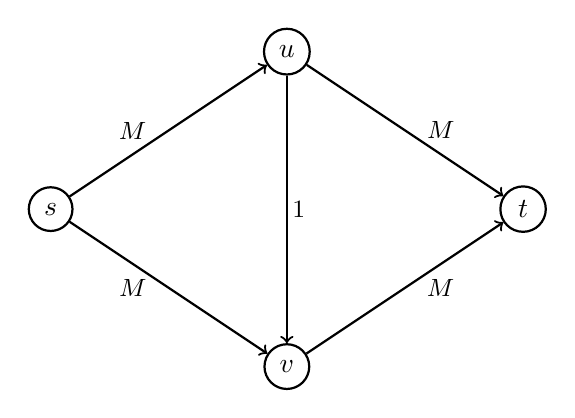
\begin{tikzpicture}[style=thick]
\tikzstyle{vertex}=[draw,shape=circle]
\tikzstyle{edge} = [draw,thick,-]
\tikzstyle{weight} = [font=\small];

\draw (0,0) node[vertex] (s) {$s$};
\draw (3,2) node[vertex] (u) {$u$};
\draw (3,-2) node[vertex] (v) {$v$};
\draw (6,0) node[vertex] (t) {$t$};

\path[edge,->] (s) -- node[weight,xshift=-3ex] {$M$} (u);
\path[edge,->] (s) -- node[weight,xshift=-3ex] {$M$} (v);
\path[edge,->] (u) -- node[weight,xshift=1ex] {$1$} (v);
\path[edge,->] (u) -- node[weight,xshift=3ex] {$M$} (t);
\path[edge,->] (v) -- node[weight,xshift=3ex] {$M$} (t);
\end{tikzpicture}
\end{center}
The example above shows that, if the augmenting paths are chosen in a
disadvantageous way, then the Ford-Fulkerson algorithm may take $\Omega(M)$
iterations, where $M$ is the largest capacity in the network. This
happens if all augmenting paths use the arc $uv$ or $vu$ respectively
in the residual network. 




\begin{corollary}[integrity theorem]
  If $u(a) \in \setN$ for each $a \in A$, then there exists an integer maximum
  flow ($f(a) \in \setN$ for all $a \in A$). 
\end{corollary}


\begin{proof}
This follows from the fact that the residual capacities remain
integral and thus the augmented flow is always integral. \qed 
\end{proof}



\begin{theorem}
\label{f:thr:10}
If we choose in each iteration a shortest $s-t$-path in $D(f)$ as a
flow-augmenting path, the number of iterations is at most $|V| \cdot|A|$. 
  
\end{theorem}

\begin{definition}
  Let $D = (V,A)$ be a digraph, $s,t \in V$  and let  $\mu(D)$ denote the
  length of a  shortest path from $s$ to $t$. Let $\alpha(D)$ denote the set
  of arcs contained in at least one shortest $s-t$ path.
\end{definition}

\begin{theorem}
  \label{f:thr:11}
  Let  $D = (V,A)$ be a digraph and  $s,t \in V$. Define $D' = (V,A \cup
  \alpha(D)^{-1})$. Then $\mu(D) = \mu(D')$ and $\alpha(D) = \alpha(D')$.
\end{theorem}


\begin{proof}
  It suffices to show that $\mu(D)$ and $\alpha(D)$ are invariant if we add
  $a^{-1}$ to $D$ for one arc $a \in \alpha(D)$. Suppose not, then there is a
  directed $s-t$-path $P_1$ traversing $a^{-1}$ of length at most
  $\mu(D)$. As $a \in \alpha(D)$ there is a path $P_2$ traversing $a$ of length
  $\mu(D)$. If we follow $P_2$  until the tail of $a$ is reached  and
  from thereon follow $P_1$, we obtain another $s-t$ path $P_3$ in $D$.
  Similarly if we follow $P_1$ until the head of $a$ is reached and then follow $P_2$,
  we obtain a fourth $s-t$ path $P_4$ in $D$. However $P_3$ or $P_4$ has length less
  than $\mu(D)$. This is a contradiction. \qed
\end{proof}


\begin{proof}[of Theorem~\ref{f:thr:10}]
  Let us augment flow $f$ along a shortest $s-t$-path $P$ in $D(f)$
  obtaining flow $f'$. The residual graph $D_{f'}$ is a subgraph of
  $D' = (V, A_f \cup\alpha(D(f))^{-1})$. Hence $\mu(D_{f'}) \geq \mu(D')=\mu(D(f))$. If
  $\mu(D_{f'})=\mu(D(f))$, then $\alpha(D_{f'})\subseteq\alpha(D') = \alpha(D(f))$. At least one
  arc of $P$ does not belong to $D_{f'}$, (the arc of minimum residual
  capacity!) thus the inclusion is
  strict. Since $\mu(D(f))$ increases at most $|V|$~times and, as long as
  $\mu(D(f))$ does not change, $|\alpha(D(f))|$ decreases at most $2\, |A|$~times, we
  have the theorem. \qed
\end{proof}

In the following let $m = |A|$ and $n = |V|$. 

\begin{corollary}
  \label{co:2}
  A maximum flow can be found in time $\bigO(n \, m^2)$.
\end{corollary}




\section{Minimum cost network flows, MCNFP}
\label{sec:minimum-cots-flows}

In contrast to the maximum $s-t$-flow problem, the goal here is to
route a flow, which comes from several sources and sinks through a
network with capacities and \emph{costs} in such a way, that the total
cost is minimized. 

\begin{example}
  Suppose you are given a directed graph $D=(V,A)$ with arc weights  
  $c: A \to \setR_{\geq0}$ and your task is to compute a shortest 
  path from a particular node $s$ to all other nodes in the graph 
  and assume that such paths exist. Then one can model this as a 
  MCNFP (minimum cost network flow problem) by sending a flow of 
  value $|V|-1$ into the source node 
  and by letting a flow of value $1$ leave each node. The costs on 
  the arcs are defined by $c$. The arcs have infinite capacities. 
  We will see later, that this MCNFP 
  has an integral solution which corresponds to the shortest
  paths from $s$ to all other nodes. 
\end{example}


\begin{figure}
  \centering
  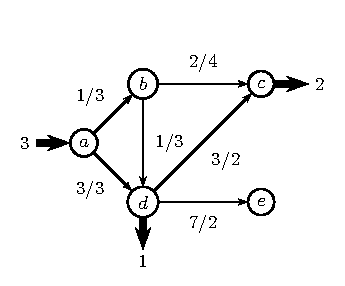
\includegraphics{figures/flows1.pdf}   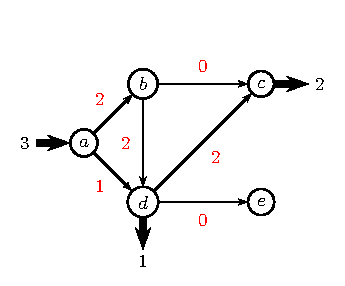
\includegraphics{figures/flows2.pdf} 
  \caption{A Network with in/out-flow, costs and capacities and a
    feasible flow of cost $13$. }
  \label{ex:net:1}
\end{figure}

 


Here is a formal definition of a MCNFP. In
this notation, vertices are indexed with the letters $i,j,k$ and arcs 
are denoted by their tail and head respectively, for example
$(i,j)$ denotes the arc from $i$ to $j$. 
  
% For a node $i\in V$, the subset $I(i)\subseteq V$ denotes the incoming nodes of
% $i$, i.e., the set $I(i) = \{ j \mid (j,i) \in A\}\subseteq V$. Similarly $O(i) = \{ j
% \mid (i,j) \in A\}\subseteq V$ denotes the set of outgoing nodes.

 A \emph{network} is now a
directed graph $D = (V,A)$ together with a capacity function $u: A \to
\setQ_{\geq0}$, a cost function $c: A \to\setQ$ and an external flow $b: V \to \setQ$.
The value of $b_i$ denotes the amount of flow which comes from the
exterior. If $b_i>0$, then there is flow from the outside, entering
the network through node $i$. If $b_i<0$, there is flow which leaves
the network through $i$.

In the following we often use the notation $f(i,j)$ for the flow-value
on the arc $(i,j)$ (instead of $f((i,j))$). Similarly we write
$c(i,j)$ and $u(i,j)$. 

A \emph{feasible flow} is a function $f:A \to \setQ_{\geq0}$ which
satisfies the following constraints. 
\begin{displaymath}  
  \begin{array}{cl}
    \sum_{e \in \delta^{out}(i)} f{(e)} - 
    \sum_{e \in \delta^{in}(i)} f(e) =b_i & 
    \text{ for all } i \in V, \\
    0 \leq f{(e)} \leq u{(e)}              & \text{ for all } e \in A.
  \end{array}
\end{displaymath}


The goal is to find a feasible flow with minimum cost: 


  \begin{displaymath}
    \begin{array}{rcl}
      \text{minimize}     & \sum_{e \in A} c(e) f(e) &     \\
      \text{ subject to}  & \sum_{e \in \delta^{out}(i)} f(e) - \sum_{e\in \delta^{in}(i)} f(e) =b_i & \text{ for all } i \in V,\\
                          & 0 \leq f(e) \leq u(e)              &
                          \text{ for all } e \in A 
    \end{array}
  \end{displaymath}
  

  \begin{example}
    Imagine you are a pilot and fly a passenger airplane in
    hops from airport $1$ to airport $2$ to airport $3$ and so on, 
    until airport $n$.  At airport $i$ there are $b_{ij}$ passengers 
    that want to travel to airport $j$, where $j>i$. You may decide 
    how many of the $b_{ij}$ passengers you will take on board. Each 
    of the passengers will pay $c_{ij}$ dollars for the trip. The 
    airplane can accommodate $p$ people. 

    You are a greedy pilot and think of a plan to pick up and deliver
    passengers on your hop from $1$ to $n$ which maximizes your
    revenue. 

    Finding this plan can be modeled as a MCNFP. 
    Your network has nodes $1,\ldots,n$ and arcs
    $(i,i+1), i=1,\ldots,n-1$ with capacities $p$ and  without
    costs. These nodes do not have  in/out-flow from   the outside. 
    You furthermore have nodes $i\to j$ for $i<j$ and 
    $i,j \in \{1,\ldots,n\}$ which are excess nodes with in-flow 
    $b_{ij}$ from the outside. Each node $i\to j$ is connected to
    $i$ and to $j$ with a directed arc. The capacities on these arcs
    are infinite. The cost of the arc $(i\to j,i)$ is $-c_{ij}$. 
    The cost of the arc $(i\to j,j)$ is zero. The outflow on the 
    node $j$ is the total number of passengers that want to fly to 
    node $j$. An integral optimal flow to this problem is an optimal 
    plan for you. 
  \end{example}


  
  Throughout this chapter we make the following assumptions.
  
  \begin{enumerate}
  \item All data (cost, supply, demand and capacity) are integral.
  \item The network contains an incapacitated directed path between
    every pair of nodes. 
  \item The supplies/demands at the nodes satisfy the condition 
    $\sum_{i \in V} b_i=0$ and the MCNFP has a feasible solution. 
  \item All arc costs are nonnegative. 
  \item The graph does not contain a pair of reverse arcs. 
  \end{enumerate}

\begin{exercise} 
   Show how to transform a MCNFP on a digraph with pairs of 
   reverse arcs into a MCNFP on a digraph with no pairs of 
   reverse arcs.  The number of arcs and nodes should 
   asymptotically remain the same.
\end{exercise}
  
  An \emph{arc-flow} of $D$ is a flow vector, that satisfies the
  nonnegativity and capacity constraints. 
 
  \begin{eqnarray*}
        \sum_{e\in \delta^{in}(i)} f(e) -  \sum_{e \in \delta^{out}(i)} f(e)  =  g(i) & &   \text{ for all } i \in V,\\
        0 \leq f(e) \leq u(e)                 & &   \text{ for all }
        e \in A. 
  \end{eqnarray*}


  \begin{itemize}
  \item  If $g(i) >0$, then $i$ is an \emph{excess node} (more inflow than
    outflow).
  \item  If $g(i) <0$, then $i$ is a \emph{deficit node} (more outflow than
    inflow).
  \item  If $g(i) = 0$ then $i$ is a \emph{balanced node}.
  \end{itemize}
  
  
\begin{exercise}
   Prove that $\sum_{i \in V} g(i) = 0$ holds and thus that a 
   feasible flow only exists if the sum of the $b(i)$ is equal 
   to zero. 
\end{exercise}

  
  Let $\paths$ be the collection of directed paths  of $D$ and
  let $\cycles$ be the collection of directed cycles of $D$. A
  path-flow is a function $\beta: \paths \cup \cycles \to \setR_{\geq0}$ which assigns
  flow values to paths and cycles. 

  For $(i,j)\in A$ and $P \in \paths$ let $\delta_{(i,j)}(P)$ be $1$ if $(i,j) \in
  P$ and $0$ otherwise. For $C \in \cycles$ let $\delta_{(i,j)}(C)$ be $1$ if
  $(i,j)\in C$ and $0$ otherwise. 

  A path-flow $\beta$ determines a unique   arc-flow
  \begin{displaymath}
    f(i,j) = \sum_{P \in \paths} \delta_{(i,j)}(P) \beta(P) + \sum_{C \in \cycles} \delta_{(i,j)}(C) \beta(C). 
  \end{displaymath}
    

  
  \begin{theorem}
    \label{f:thr:Decomp}
    Every path and cycle flow  has a unique representation
    as a  nonnegative arc-flow. Conversely, every nonnegative arc-flow
    $f$ can be represented as a path and cycle flow with the following
    properties:
    \begin{enumerate}
    \item Every directed path with positive flow connects a deficit
      node with an excess node.
    \item At most $n+m$ paths and cycles have nonzero flow and at most
      $m$ cycles have nonzero flow.
    \end{enumerate}
    If the arc-flow $f$ is integral, then so are the path and cycle
    flows into which it decomposes. 
  \end{theorem}

  \begin{proof}
   
  
  ``$\Rightarrow$'' See discussion above.
  
  ``$\Leftarrow$'' 
  
  Let $f$ be an arc-flow. Suppose $i_0$ is a deficit node. Then there
  exists an incident arc $(i_0,i_1)$ which carries a positive flow. If
  $i_1$ is an excess node, we have found a path from deficit to excess
  node. Otherwise, the flow balance constraint at $i_1$ implies that
  there exists an arc $(i_1,i_2)$ with positive flow. Repeating this
  procedure, we finally must arrive at an excess node or revisit a
  node. This means that we either have constructed a directed path $P$
  from deficit node to excess node or a directed cycle $C$, both
  involving only arcs with strictly positive flow.
  
  In the first case, let $P = i_0,\ldots,i_k$ be the directed path from
  deficit node $i_0$ to excess node $i_k$. We set $\beta(P) =
  \min\{-e_{i_0}, e_{i_k}, \min\{f{(i,j)} \mid (i,j) \in P\} \}$ and $f{(i,j)} =
  f{(i,j)} - \beta(P), \, (i,j) \in P$.  In the second case, set $\beta(C) =
  \min\{f{(i,j)} \mid (i,j) \in C$ and $f{(i,j)} = f{(i,j)} - \beta(C), \, (i,j)
  \in C$.  Repeat this procedure until all node imbalances are zero.
  
  Now find an arc with positive flow and construct a cycle $C$ by
  following only positive arcs from there. Set 
  $\beta(C) = \min\{f{(i,j)} \mid  (i,j) \in C\}$ and 
  $f{(i,j)} = f{(i,j)} - \beta(C),\, (i,j) \in C\}$. Repeat this process until
  there are no positive flow-arcs left. 

  Each time a path or a cycle is identified, the excess/deficit of
  some node is set to zero or some arc is set to zero. This implies
  that we decompose into at most $n+m$ paths and cycles. Since cycle
  detection sets an arc to zero we have at most $m$ cycles.  \qed
\end{proof}
  
  An arc flow $f$ with $g(i)=0$ for each $i \in V$ is called a
  \emph{circulation}. 
  
  \begin{corollary}
    A circulation can be decomposed into at most $m$ cycle-flows.
  \end{corollary}

  
  Let $D = (V,A)$ be a network with capacities 
  $u{(i,j)}, \,  (i,j) \in A$ and costs $c{(i,j)}, \, (i,j) \in A$ and let
  $f$ be a feasible flow of the network. The \emph{residual network} $D(f)$ is
  defined as follows.

  \begin{itemize}
  \item We replace each arc $(i,j) \in A$ with two arcs $(i,j)$ and
    $(j,i)$.
  \item The arc $(i,j)$ has cost $c{(i,j)}$ and \emph{residual capacity}
    $r{(i,j)} = u{(i,j)} - f{(i,j)}$.  
  \item The arc $(j,i)$    has cost $-c{(i,j)}$ and
    residual capacity $r{(j,i)}=f{(i,j)}$. 
  \item      Delete all arcs which do not have strictly positive residual
    capacity. 
  \end{itemize}

  

  \begin{figure}
  \centering
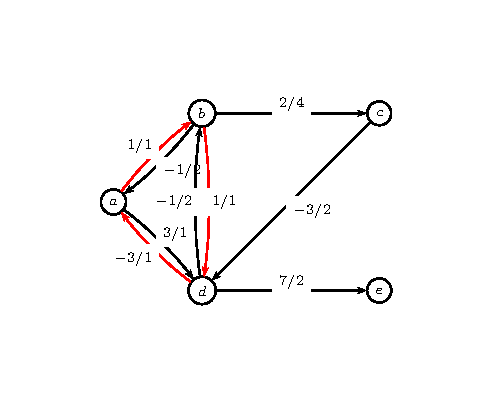
\includegraphics{figures/flows6.pdf}
\caption{The residual network of the flow in Figure~\ref{ex:net:1} and
a negative cycle marked by the red edges.} \label{ex:net:2}
\end{figure}



  A directed cycle (or path) in $D(f)$ is called an 
  \emph{augmenting cycle (or path)} of $f$.  

 
  \begin{lemma}
    \label{lem:6}
    Suppose that $f$ and $f^\circ$ are feasible flows, then 
    $f  - f^\circ$  is a circulation in $D(f^\circ)$.  Here $f  -
    f^\circ$ is the flow  
    \begin{displaymath}
      (f-f^\circ)(e) = 
      \begin{cases}
        \max\{0, f(e) - f^\circ(e)\}, & \text{ if } e \in  A(D)\\
        \max\{0, f^\circ(e) - f(e)\}, & \text{ if } e^{-1} \in  A(D)\\
        0, & \text{ otherwise.}
      \end{cases}
    \end{displaymath}
  \end{lemma}
   
  


  \begin{proof}
    It is very easy to see that the flow $f - f^\circ$ satisfies the
    capacity constraints. One also has for each $v \in V$
    \begin{displaymath}
      \sum_{e \in \delta^{out}(v)} (f (e) - f^\circ(e))  - \sum_{e \in \delta^{in}(v)}
      (f (e) - f^\circ(e)) = 0.
    \end{displaymath}
    If a term $(f (e) - f^\circ(e))$ is negative, it is replaced by its
    absolute value and charged as flow on the arc $e^{-1}$ in
    $D(f^\circ)$ which leaves its contribution to the sum above
    invariant. 
    \qed     
  \end{proof}




  \begin{figure}
  \centering
% \psset{unit=1.5cm}  
 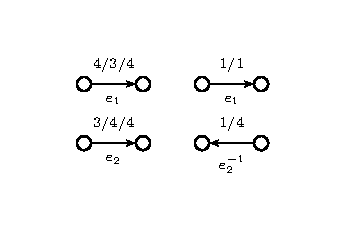
\includegraphics{figures/flows4.pdf}
\caption{Two  arcs $e_1,e_2 \in A$ labeled with $f(e)/f^\circ(e)/u(e)$ and the
  corresponding flow on these arcs (or their reverse) in
  $D(f^\circ)$. Arcs in $D(f^\circ)$ are labeled with flow and capacity
  values respectively. }\label{fig:diff}
\end{figure}


  \begin{theorem}[Augmenting Cycle Theorem]
    \label{f:thr:augcyc}
    Let $f$ and $f^\circ$ be any two feasible flows of a network flow
    problem. Then $f$ equals $f^\circ$ plus the flow of at most $m$
    directed cycles in $D(f^\circ)$.  Furthermore the cost of $f$ equals
    the cost of $f^\circ$ plus the cost of flow on these augmenting
    cycles. 
  \end{theorem}
  
  \begin{proof}
    This can be seen by applying flow decomposition on the  flow 
    $f - f^\circ$  in $D(f^\circ)$. \qed
  \end{proof}
  

 
  
  \begin{theorem}[Negative Cycle Optimality Conditions]
    \label{f:thr:13}
    A feasible flow $f^*$ is an optimal solution of the MCNFP, 
    if and only if it satisfies the negative
    cycle optimality conditions: the residual network $D(f^*)$
    contains no directed cycle of negative cost.    
  \end{theorem}

  \begin{proof}
    

  ``$\Rightarrow$'' Suppose that $f$ is a feasible flow and that $D(f)$ contains
  a negative directed cycle. Then $f$ cannot be optimal, since we can
  augment positive flow along the corresponding cycle in the
  network. Therefore, if $f^*$ is an optimal flow, then $D(f^*)$
  cannot contain a negative directed cycle. 

  ``$\Leftarrow$'' Suppose now that $f^*$ is a feasible flow and suppose that
  $D(f^*)$ does not contain a negative cycle. Let $f^\circ$ be an optimal
  flow with $f^\circ \neq f^*$. The vector $f^\circ-f^*$ is a circulation in
  $D(f^\circ)$ with
  non-positive cost $c^T(f^\circ-f^*) \leq0$. It follows from
  Theorem~\ref{f:thr:augcyc} that the cost of $f^\circ$ equals the cost of
  $f^*$ plus  the cost of directed cycles in the residual network
  $D(f^*)$.  The cost of these cycles is nonnegative, and therefore
  $c(f^\circ) \geq c(f^*)$ which implies that $f^*$ is optimal. 
  \qed
\end{proof}




\begin{figure}
  \centering
  
  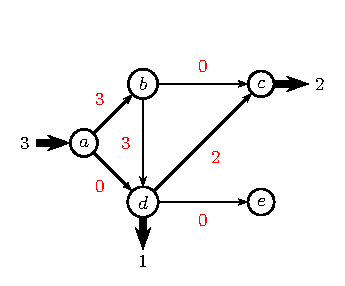
\includegraphics{figures/flows5.pdf} 
\caption{The result of augmenting a flow of one along the negative
  cycle in Figure~\ref{ex:net:2}. This flow has cost 12 but is not
  optimal, since the residual network still contains a negative
  cycle.}\label{ex:net:3}
\end{figure}





\begin{algorithm}[Cycle Canceling Algorithm]
  \label{alg:1}
  ~\\
  \begin{enumerate}
  \item  establish a feasible flow $f$ in the network
  \item {\tt WHILE} $D(f)$ contains a negative cycle
    \begin{enumerate}
    \item  detect a negative cycle $C$ in $D(f)$
    \item let $\delta=\min\{r{(i,j)} \mid (i,j) \in C\}$
    \item augment $\delta$ units of flow along the cycle $C$
    \item update $D(f)$
    \end{enumerate}
  \item {\tt RETURN}  $f$
  \end{enumerate}
\end{algorithm}




  \begin{theorem}
    \label{f:thr:12}
    The cycle canceling algorithm terminates after a finite number of
    steps if the MCNFP has an optimal solution. 
  \end{theorem}
  \begin{proof}   
  The cycle canceling algorithm reduces the cost in each iteration.
  We have assumed that the input data is integral. Thus the cost
  decreases by at least one unit each iteration. 
  Therefore the number of iterations is finite.    
  \qed
\end{proof}


\begin{corollary}
  \label{co:3}
  If the capacities are  integral and if the MCNFP has a optimal flow, then
  it has an optimal flow with integer values only. 
\end{corollary}



%Consider the MCNFP

%\begin{displaymath}
%    \begin{array}{rcl}
%      \text{minimize}     & \sum_{(i,j) \in A} c{(i,j)} f{(i,j)} &     \\
%      \text{ subject to}  & \sum_{j \in O(i)} f{(i,j)} - \sum_{j\in I(i)} f{(j,i)} =b_i & \text{ for all } i \in V,\\
%                          & 0 \leq f{(i,j)} \leq u{(i,j)}              & \text{ for all } (i,j) \in A.
%    \end{array}
%  \end{displaymath}
    

%We transform this problem into standardform via slackvariables 
%$z{(i,j)}\geq0,\, (i,j) \in A$:

%\begin{displaymath}
%    \begin{array}{rrcll}
%      \text{minimize}     & \sum_{(i,j) \in A} c{(i,j)} f{(i,j)} &     \\
%      \text{ subject to}  & \sum_{j \in O(i)} f{(i,j)} - \sum_{j\in I(i)} f{(j,i)}
%      & = & b_i & \text{ for all } i \in V,\\
%                          & f{(i,j)} + z{(i,j)} & = &  u{(i,j)}
%                          & \text{ for all } (i,j) \in A, \\
%                    & f{(i,j)},z{(i,j)} & \geq & 0. &       \\
%    \end{array}
%  \end{displaymath}



  
%  The dual of this problem has variables $\pi_i, \, i \in V$ and 
%  $\alpha{(i,j)},  \,(i,j) \in A$ and is defined as follows:
  
  
%  \begin{displaymath}
%    \begin{array}{rrcll}
%      \text{maximize}     & \sum_{i \in V} b_i \pi_i  - \sum_{(i,j) \in A} u{(i,j)} \alpha{(i,j)}      \\
%      \text{ subject to}  & \pi_i - \pi_j - \alpha{(i,j)} 
%      & \leq & c{(i,j)} & \text{ for all } (i,j) \in A,\\
%                          & \alpha{(i,j)} & \geq & 0
%                          & \text{ for all } (i,j) \in A.
%  \end{array}
%  \end{displaymath}


Let $\pi : V  \to \setR$ be a function (\emph{node potential}). The
\emph{reduced cost} of an arc $(i,j)$ w.r.t. $\pi$ is 
$c_\pi((i,j))=c((i,j))+\pi(i) - \pi(j)$. The potential $\pi$ is called
\emph{feasible} if $c_\pi((i,j))\geq0$ for all arcs $(i,j)\in A$. 

\begin{lemma}
  \label{lem:7}
  Let $D = (V,A)$ be a digraph with arc weights $c:A\to\setR$. Then $D$
  does not have a negative cycle if and only if there exists a
  feasible node potential $\pi$ of $D$. 
\end{lemma}


\begin{proof}
  Consider a directed path $P = i_0,i_1,\ldots,i_k$. The cost of this
  path is 
  \begin{displaymath}
    c(P) = \sum_{j=1}^{k}c((i_{j-1},i_j)).
  \end{displaymath}
  The reduced cost of this path is equal to 
  \begin{displaymath}
    c_\pi(P) = \sum_{j=1}^{k}c((i_{j-1},i_j)) + \pi(i_0) - \pi(i_k).
  \end{displaymath}
  If $P$ is a cycle, then $i_0$ and $i_k$ are equal, which means that
  its cost and reduced cost coincide. Thus, if there exists a feasible
  node potential, then there does not exist a negative cycle. 

  
  On the other hand, suppose that $D$ does not contain a negative
  cycle w.r.t. $c$. Add a vertex $s$ to $D$ and the arcs $(s,i)$ for all 
  $i \in  V$. The weights (costs) of all these new arcs is $0$. Notice
  that in this way, no new cycles are created, thus still there does
  not exist a negative cycle. This means we can compute the shortest
  paths from $s$ to all other nodes $i \in V$. Let $\pi$ be the function
  which assigns these shortest paths lengths. Clearly $c_\pi((i,j)) =
  \pi(i) - \pi(j) + c((i,j))\geq0$, since the shortest-path length to $j$ is
  at most the shortest-path length to $i$ plus $c((i,j))$.  \qed
\end{proof}

  
This means that we have again a nice way to prove that a flow is
optimal. Simply equip  the residual network with a feasible node
potential.  



\begin{corollary}[Reduced Cost Optimality Condition]
  \label{co:1}
  A feasible flow $f^*$ is optimal if and only if there exists a node
  potential $\pi$ such that the reduced costs $c_\pi{(i,j)}$ of  each arch
  $(i,j)$ of $D(f)$ are nonnegative. 
\end{corollary}






  The cycle canceling algorithm is only pseudopolynomial. If we could
  always chose a minimum cycle (cycle with best improvement) as an
  augmenting cycle, we would have a polynomial number of
  iterations. Finding minimum cycles is $NP$-hard. Instead we augment
  along \emph{minimum mean cycles}. One can find minimum mean cycles
  in polynomial time.  

  The \emph{mean cost} of a cycle $C \in \cycles$ is the cost of $C$
  divided by the number of arcs in $C$:
  \begin{displaymath}
    \sum_{(i,j) \in C} c{(i,j)})  / |C|.
  \end{displaymath}
  

  \begin{algorithm}[Minimum Mean Cycle Canceling, MMCC]
    \label{alg:2}
    ~\\
    \begin{enumerate}
    \item establish a feasible flow $f$ in the network
    \item {\tt WHILE} $D(f)$ contains a negative cycle
      \begin{enumerate}
      \item  detect a minimum mean cycle $C$ in $D(f)$ 
      \item   $\delta=\min\{r{(i,j)} \mid (i,j) \in C\}$
      \item   augment $\delta$ units of flow along the cycle $C$
      \item   update $D(f)$ 
      \end{enumerate}
    \item {\tt RETURN} $f$
    \end{enumerate}
  \end{algorithm}



  We now analyze the MMCC-algorithm. Let $\mu(f)$ denote the minimum
  mean-weight of a cycle in $D(f)$. 
  
  \begin{lemma}[See Korte \& Vygen \cite{MR1897297}]
    \label{lem:8}
    Let $f_1,f_2,\ldots$ be a sequence of feasible flows such that
    $f_{i+1}$ results from $f_i$ by augmenting flow along $C_i$, where
    $C_i$ is a minimum mean cycle of $D(f_i)$, then
    \begin{enumerate}
    \item \label{item:5} $\mu(f_k)\leq\mu(f_{k+1})$ for all $k$.
    \item \label{item:6} $\mu(f_k) \leq \frac{n}{n-1} \mu(f_l)$, where $k<l$
      and $C_k \cup C_l$ contains a pair of reversed arcs.
    \end{enumerate}
  \end{lemma}



  \begin{proof}
    
    \ref{item:5}): Suppose $f_k$ and $f_{k+1}$ are two subsequent flows in this
    sequence. Consider the multi-graph $H$ which results from $C_k$
    and $C_{k+1}$ by deleting pairs of opposing arcs.  The arcs of
    $H$ are a subset of the arcs of $D(f_k)$, since an arc of
    $C_{k+1}$ which is not in $D(f_k)$ must be a reverse arc of $C_k$.

    Each node in $H$ has even degree.  Thus $H$ can be
    decomposed into cycles, each of mean weight at least $ \mu(f_k)$.  
    Thus we have $c(A(H)) \geq \mu(f_k) |A(H)|$. 

    Since the total weight of each reverse pair of arcs is zero we
    have 
    \begin{displaymath}
      c(A(H)) = c(C_k) + c(C_{k+1}) = \mu(f_k) |C_k|   + \mu(f_{k+1}) |C_{k+1}|.
    \end{displaymath}

    Since $|A(H)| \leq |C_k| + |C_{k+1}|$ we conclude 
    \begin{eqnarray*}
       \mu(f_k) ( |C_k| + |C_{k+1}|) & \leq &  \mu(f_k)|A(H)| \\
                              & \leq & c(A(H)) \\
                              & = & \mu(f_k) |C_k|   + \mu(f_{k+1}) |C_{k+1}|.
    \end{eqnarray*}

    Thus $\mu(f_k) \leq \mu(f_{k+1})$. 

    
    \ref{item:6}): By the first part of the theorem, it is enough to
    prove the statement for $k,l$ such that $C_i \cup C_l$ does not
    contain a pair of reverse arcs for each  $ i, \, k < i < l$.  

    Again, consider the graph $H$ resulting from  $C_k$
    and $C_{l}$ by deleting pairs of opposing arcs. $H$ is a subgraph
    of $D(f_k)$, since any arc of $C_l$ which does not belong to
    $D(f_k)$ must be a reverse arc of $C_k,C_{k+1},\ldots,C_{l-1}$. But
    only $C_k$ contains a reverse arc of $C_l$. So as above we have 
    \begin{displaymath}
      c(A(H)) = c(C_k) + c(C_{l}) = \mu(f_k) |C_k|   + \mu(f_{l})      |C_{l}|. 
    \end{displaymath}
    
    Since $|A(H)| \leq |C_k| + |C_{l}| -2$ we have $|A(H)| \leq
    \frac{n-1}{n}( |C_k| + |C_{l}|)$. Thus we get
    \begin{eqnarray*}
       \mu(f_k)\frac{n-1}{n} ( |C_k| + |C_{l}|) & \leq &  \mu(f_k)|A(H)| \\
                              & \leq & c(A(H)) \\
                              & = & \mu(f_k) |C_k|   + \mu(f_{l})|C_{l}|\\          
                              & \leq & \mu(f_{l}) (|C_k|   + |C_{l}|) \\                       
    \end{eqnarray*}
    This implies that $\mu(f_k) \leq \frac{n}{n-1}  \mu(f_l)$.  
    \qed
  \end{proof}






  \begin{corollary}
    \label{co:4}
    During the execution of the MMCC-algorithm, $|\mu(f)|$ decreases by
    a factor of $1/2$ every $n\cdot m$ iterations. 
  \end{corollary}

  \begin{proof}
    Let $C_1, C_2,\ldots$ be the sequence of augmenting cycles. Every
    $m^{th}$ iteration, there must be an arc of the cycle, which is
    reverse to one of the succeeding $m-1$ cycles, because every
    iteration, one arc of the residual network will be deleted. 
    Thus after $n \, m$ iterations, the absolute value of $\mu$ has
    dropped by $\left(\frac{n-1}{n} \right)^n \leq e^{-1} \leq 1/2$.  \qed
  \end{proof}

  \begin{corollary}
    \label{co:5}
    If all data are integral, then the
    MMCC-algorithm runs in polynomial time. 
  \end{corollary}
  
  \begin{proof}
    \begin{itemize}
    \item A lower bound on $\mu$ is the smallest cost $c_{min}$
    \item $|\mu|$ drops by $1/2$ every $m \, n$ iterations. 
    \item After $m n \log n |c_{min}|$ iterations, absolute value
    of minimum mean weight cycle   drops below $1/n$, thus is zero.
    \item {\bf We need to prove that a minimum mean cycle can be found        in polynomial time} 
    \end{itemize} \qed
  \end{proof}


This is a so-called \emph{weakly polynomial} bound, since the binary
encoding length of the numbers in the input (here the costs)
influences the running time. We now prove that the MMCC-algorithm is
\emph{strongly polynomial}. 






\begin{theorem}[See Korte \& Vygen~\cite{MR1897297}]
  The MMCC-algorithm requires  $\bigO(m^2 \, n \log n)$ iterations
  (mean weight cycle cancellations). 
\end{theorem}

\begin{proof}
  One shows that every $m\, n  (\lceil\log n\rceil+1)$ iterations, at least one
  arc is \emph{fixed}, which means that the flow through  this arc
  does not change anymore. 
  
  Let $f_1$ be some flow at some iteration and let $f_2$ be the flow
  $m\, n  (\lceil\log n\rceil+1)$ iterations later. 
  It follows from Corollary~\ref{co:4} that 
  \begin{equation}
    \label{f:eq:33}
    \mu(f_1)\leq 2 \, n \, \mu(f_2) 
  \end{equation}
  %
  holds. 
  
  Define the costs $c'(e) = c(e) - \mu(f_2)$ for the residual network
  $D(f_2)$. There exists no negative cycle in $D(f_2)$ w.r.t. this
  cost $c'$. (A cycle $C$ has weight $c'(C) = \sum_{e\in C} c(e) - |C|
  \mu(f_2)$ and thus $c'(C) / |C| = \sum_{e\in C} c(e) / |C| - \mu(f_2)\geq0$).
  By Lemma~\ref{lem:7} there exists a feasible node potential $\pi$ for
  these weights. One has $0 \leq c'_\pi(e) = c_\pi(e) - \mu(f_2)$ and thus
  \begin{equation}
    \label{f:eq:32}
     c_\pi(e) \geq \mu(f_2), \text{ for all } e \in A(D(f_2)). 
  \end{equation}

  Let $C$ be a minimum mean cycle of $D(f_1)$. One has
  \begin{equation}
    \label{f:eq:34}
    c_\pi(C) = c(C) = \mu(f_1) \, |C| \leq 2 \, n \, \mu(f_2) |C|.
  \end{equation}
  
  It follows that there exists an arc $e_0$ of $C$ such that
  \begin{equation}
    \label{f:eq:36}
    c_\pi(e_0)\leq 2 \, n \, \mu(f_2)
  \end{equation}
  %
  holds. The inequalities~\eqref{f:eq:32}
  imply that  $e_0 \notin A(D(f_2))$ 

  We now make the following
  claim:
  %
  \begin{quote}
    Let $f'$ be a feasible flow such that $e_0 \in D(f')$, then 
    $\mu(f') \leq    \mu(f_2)$. 
  \end{quote}
  
  If we have shown this claim, then it follows from Lemma~\ref{lem:8}
  that $e_0$ cannot be anymore in the residual network of a flow after
  $f_2$.  Thus the flow along the arc $e_0$ (or $e_0^{-1}$) is
  fixed. 

  Let $f'$ be a flow such that $e_0\in A(D(f'))$. Recall that $f' - f_2$
  is a circulation in $D(f_2)$ where $e_0\notin D(f_2), \,e_0^{-1}\in D(f_2)$  and this
  circulation sends flow over $e_0^{-1}$. This circulation can be
  decomposed into cycles and one of these cycles $C$ contains
  $e_0^{-1}$.  One has $c_\pi(e_0^{-1}) = -c_\pi(e_0) \geq -  2 \, n \,
  \mu(f_2)$ (eq.~\eqref{f:eq:36}). Using~\eqref{f:eq:32} one obtains
  \begin{eqnarray}
    \label{f:eq:37}
    c(C) & = &  \sum_{e \in C} c_\pi(e) \\
         & \geq &  -  2 \, n \,  \mu(f_2) + (n-1) \mu(f_2) \\
         & = & - (n +1)\, \mu(f_2) \\
         & > & -n \, \mu(f_2). 
  \end{eqnarray}
  %
  The reverse of $C$ is an augmenting cycle for $f'$ with total weight
  at most $n \, \mu(f_2)$ and thus with mean weight at most
  $\mu(f_2)$. Thus $\mu(f') \leq \mu(f_2)$.  \qed
\end{proof}






\section{Computing a minimum cost-to-profit ratio cycle}
\label{sec:comp-minim-cost}

Given a digraph $D = (V,A)$ with costs $c:A\to\setZ$ and profit $p:A \to
\setN_{>0}$, the task is to compute a cycle $C \in \cycles$ with minimum
ratio 
\begin{equation}
  \label{f:eq:31}
  \frac{c(C)}{p(C)}.
\end{equation}

Notice that this is the largest number $\beta\in \setQ$ which satisfies 
\begin{equation}
  \beta\leq  \frac{c(C)}{p(C)}, \, \text{ for all } C \in \cycles. 
\end{equation}

By rewriting this inequality, we understand this to be the largest
number $\beta\in \setQ$ such that 
\begin{equation}
  c(C) - \beta\, p(C) \geq0 \, \text{ for all } C \in \cycles. 
\end{equation}
In other words, given a digraph $D= (V,A)$ with costs 
$c_\beta:A \to \setQ$, where $c_\beta(e) = c(e) - \beta\,p(e)$,
we search the largest number $\beta \in \setQ$ such that the
\begin{equation}
   c_{\beta} \geq 0.
\end{equation}

We need a routine to check whether $D$ has a negative cycle for a
given weight function $c$. For this we assume w.l.o.g. that each 
vertex is reachable from the vertex $s$, if necessary by introducing a
new vertex $s$ from which there is an arc with cost and profit $0$ to
all other nodes. The minimum cost-to-profit ration cycle w.r.t. this
new graph is then the minimum cost-to-profit ratio cycle w.r.t. the
original graph, since $s$ is not a vertex of any cycle. 

Recall the following single-source shortest-path algorithm  of
Bellman-Ford which we now apply with weights $c_\beta$: 


{\small
  \begin{quote}
    Let $n=|V|$ and $m=|A|$. We calculate functions 
    $f_0,f_1,\ldots,f_n:V\longrightarrow\setR\cup\{\infty\}$
    successively by the following rule. 
    
    \begin{enumerate}[i)]
    \item $f_0(s) = 0$, $f_0(v) = \infty$ for all $v \neq s$ 
    \item For $k<n$ if $f_k$ has been found, compute 
      \begin{displaymath}
        \displaystyle f_{k+1}(v) = \min\{f_k(v), \min_{(u,v)\in A}\{f_k(u)+c_\beta(u,v)\}  
      \end{displaymath}
      for all $v \in V$. 
    \end{enumerate}
  \end{quote}
}

As seen when we talked about the Bellman-Ford algorithm, there 
exists a negative cycle w.r.t. $c_\beta$ if and only if 
$f_n(v) <f_k(v)$  for some $v \in V$ and $1\leq k<n$. Thus we can 
test in $O(m\cdot n)$ steps whether $D$ contains a 
negative cycle w.r.t. $c_\beta$. 

We now apply the following idea to  search for the correct value of
$\beta$. We keep an interval $I = [L,U]$ with the invariant that the
value  $\beta$ that we are searching lies in this interval $I$. As
starting values, we can chose $L = c_{min}$ and $U = c_{max}$, 
where $c_{min}$ and $c_{max}$ are the smallest and largest cost
respectively. In one iteration we compute $M = (L + U) /2$. We then
check whether $D$, together with $c_M$ contains a negative cycle. If
yes, we know that $\beta$ is at least $M$ and we set $L\gets M$. If not, then
$\beta$ is at most $M$ and we update the upper bound $U \gets M$. 

When can we stop this procedure? We can stop it, if we can assure that
only one valid cost-to-profit ratio cycle  lies in $[L,U]$. Suppose that $C_1$
and $C_2$ have different cost-to-profit ratios. Then 
\begin{eqnarray}
 | c(C_1) /  p(C_1) - c(C_2)/ p(C_2) | & = & \left| \frac{c(C_1)\, p(C_2) -
 c(C_2)p(C_1)}{  p(C_1) \, p(C_2)}\right| \\
                                & \geq & 1/ (n^2 p_{max}^2). 
\end{eqnarray}
%
Thus we can stop our process, if $U-L< 1/ (n^2 p_{max}^2)$, since we
know then that there can be only one cycle $c \in \cycles$ with
$c(C)/p(C) \in [L,U]$.

Suppose that $[L,U]$ is the final interval. 
We know then that 
\begin{displaymath}
  L \leq c(C) / p(C) \text{ for all } C \in \cycles 
\end{displaymath}
and 
\begin{displaymath}
  U> c(C)/p(C) \text{ holds for some } C \in \cycles. 
\end{displaymath}
Let $C$ be a minimum weight cycle w.r.t. the arc costs $c_L$. Clearly
$ U > c(C)/p(C) \geq L$ holds and thus $C$ is the minimum cost-to-profit
cycle we have been looking for. 

Let us analyze the number of required iterations. We need to halve the
starting interval-length $2 \, c$, where $c$ is the largest absolute
value of a cost, until the length is at most $1/ (n^2 p_{max}^2)$. 
We search the minimal $i\in \setN$ such that
\begin{equation}
  \label{f:eq:35}
  (1/2)^i c \leq 1/(n^2 p_{max}^2).
\end{equation}
This shows us that we need $\bigO(\log( c \,p_{max}^2 n^2))$
iterations which is $\bigO(\log n \log K)$, where $K$ is the largest
absolute value of a cost or a profit. 



\begin{theorem}[Lawler~\cite{MR0439106}]
  \label{f:thr:15}
  Let $D$ be a digraph  with costs $c:A\to\setZ$ and profit $p: A\to \setN_{>0}$
  and let $K \in \setN$   such that $|c(e)| + |p(e)| \leq K$ for all $e \in \setN$. A
  minimum cost-to-profit ratio cycle of $G$ can be computed in time
  $\bigO(m\,n \, \log n\, \log K)$.
\end{theorem}



But we knew a weakly polynomial algorithm for MCNFP from the
exercises. So you surely ask: Can we do better for minimum
cost-to-profit cycle computation? The answer is ``Yes''!



\subsection{Parametric search} 
\label{sec:parametric-search}




Let us first roughly describe  the  idea on  how to obtain a
strongly polynomial algorithm, see~\cite{Megiddo79}.  The Bellman-Ford
algorithm tells us whether our  current $\beta$ is too large or too
small, depending on whether $D$ with weights $c_\beta$ contains a
negative cycle or not. Recall that the B-F algorithm computes labels
$f_i(v)$ for $v \in V$ and $1\leq i\leq n$.  If these labels are computed
with costs $c_\beta$, then they are \emph{piecewise linear} functions in
$\beta$ and we denote them by $f_i(v)[\beta]$. 

Denote the optimal $\beta$ that we look for by $\beta^*$ and suppose that we
know an interval $I$ with such that $\beta^* \in I$ and each function
$f_i(v)[\beta]$ is linear if it is restricted to this domain $I$. Then we
can determine $\beta^*$ as follows.

Let $I = [L,U]$ be the interval and  remember that we are searching for the
largest value of $\beta \in I$ such that $f_{n}(v)[\beta]=f_{n-1}(v)[\beta]$
holds for each $v \in V$. Clearly this holds for $\beta = L$. Thus we only
need to check whether $\beta = U$ by computing the values $f_{n}(v)[U]$
and $f_{n-1}(v)[U]$ for each $v \in V$ and check whether one of these
pairs consists of different numbers. 


The idea is now to compute such an interval $I = [L,U]$ in strongly
polynomial time. 

Consider the function $f_1(v)[\beta]$. Clearly one has 
\begin{displaymath}
f_1(v)[\beta] = 
  \begin{cases}
    c(s,v) - \beta \cdot p(s,v) &  \text{ if } (s,v)\in A, \\
    \infty                  & \text{ otherwise}. 
  \end{cases}
\end{displaymath}

This shows that $f_1(v)[\beta]$ is a linear function in $\beta$ for each $v
\in V$. 

Now suppose that $i\geq1$ and that we have computed an interval
$I=[L,U]$ with  $\beta^*\in I$ and each function $f_i(v)[\beta]$ is a linear
function if $\beta$ is restricted to $I$. 

Now consider the function  $f_{i+1}(v)[\beta]$ for a particular $v \in
V$. Recall the formula 
\begin{equation}
  \label{f:eq:1}
  f_{i+1}(v)[\beta] = \min\{ f_i(v)[\beta], \min_{(u,v)\in A} \{ f_i(u)[\beta] +
  c(u,v) - \beta \cdot p(u,v)\} \}. 
\end{equation}


Each of the functions $ f_i(v)[\beta]$ and $ f_i(u)[\beta] +  c(u,v) - \beta
\cdot p(u,v)$  are linear on $I$.  The function $f_i(v)[\beta]$ can be retrieved by
computing a shortest path $P_i(v)$ from $s$ to $v$ with arc weights $c_\beta$ for
some $\beta$ in $(L,U)$ which uses at most $i$ arcs. If $\beta$ is then
allowed to vary, the line which is defined by $f_i(v)[\beta]$ on $I$ is
then the length of this path $P$   with parameter $\beta$.  Similarly we
can retrieve the functions (lines) $ f_i(u)[\beta] +  c(u,v) - \beta
\cdot p(u,v)$  for each $(u,v) \in A$. With the Bellman-Ford algorithm,
this amounts to a running time of $O(m \cdot n)$. 

We now have $n$ lines and can now compute the lower envelope of these
lines in time $O(n \log n)$ alternatively we can also compute all
intersection points of these lines and sort them w.r.t. increasing
$\beta$-coordinate. This would amount to $O(n^2 \log n)$.
Let $\beta_1,\ldots,\beta_k$ be the sorted list of  these  $\beta$-coordinates.
Now  $\beta_{trial}:= \beta_{\lfloor k/2\rfloor}$ and
check whether $\beta^*>\beta_{trial}$. If yes, we can replace $L$ by
$\beta_{trial}$ and we can delete the numbers
$\beta_1,\ldots,\beta_{\lfloor k/2\rfloor-1}$. Otherwise, we replace $U$ by $\beta_{trial}$ and
delete $\beta_{\lfloor k/2\rfloor+1},\ldots,\beta_k$. In
any case, 
we halved the number of possible $\beta$-coordinates and continue in this
way.  Such a check requires a negative cycle test in the graph
$D$ with arc weights $\beta_{trial}$ and costs $O(m \cdot n)$. In the end we have two consecutive $\beta$-coordinates and have an
interval $[L,U]$ on which  $f_{i+1}(v)[\beta]$ is linear.  To  find
an interval $I$ such that $f_{i+1}(v)[\beta]$ is linear on $I$ and $\beta^*
\in I$ costs thus $O(m \cdot n \log n)$ steps. 


We now continue to tighten \emph{this interval} such that all functions
$f_{i+1}(v)[\beta], v \in V$ are linear on $[L,U]$.  Thus in step $i+1$ this
amounts to a running time of 
\begin{displaymath}
  O\left(n \cdot ( m \cdot n \log n) \right). 
\end{displaymath}

The total running time  is thus 
\begin{displaymath}
  O(n^3 \cdot m \cdot \log n).  
\end{displaymath}

\begin{theorem}
  \label{f:thr:2}
  Let $D=(V,A)$ be a directed graph and let $c: A \longrightarrow\setR$ and
  $p:A\longrightarrow\setR_{>0}$ be functions. One can compute a cycle $C$ of $D$
  minimizing $c(C)/p(C)$ in time  $O(n^3 \cdot m \cdot \log n)$.  
\end{theorem}




\subsubsection{Exercises}

\begin{enumerate}[1)]
\item Show that there are no two different paths from $r$ to another
  node in a directed  tree $T = (V,A)$.  
\item Prove Lemma~\ref{lem:18}. 
\item  
    Why can we assume without loss of generality  that a minimum cost
    network has      a path from $i$ to $j$ for      all $i\neq j\in V$
    which is incapacitated? 
\item 
    Provide an example of a MCNFP for which the simple cycle-canceling
    algorithm from above can require an exponential number of
    cancels, if the cycles are chosen in a disadvantageous way. 
\item   Provide a proof of Theorem~\ref{f:thr:9}. 
\item Let $Q = <u_1,\ldots,u_k>$ be the queue before an iteration of the
  {\bf while} loop of the breadth-first-search algorithm. Show that
  $D[u_i]$ is monotonously increasing and that $D[u_1]+1\geq D[u_k]$. 
  Conclude that the sequence of assigned  labels (over time) is a
  monotonously increasing sequence. \label{item:16}
\item Extend the definitions and properties of flows and networks 
      in a multi-source and multi-sink network. Show that any flow 
      in a multi-source and multi-sink network corresponds to a 
      flow of identical value in the single-source and 
      single-sink network obtained by unifying the sources and 
      sinks in a single super-source and super-sink respectively.
\end{enumerate}



%%% Local Variables: 
%%% mode: latex
%%% TeX-master: "lecture"
%%% End: 
